\documentclass[11pt,aspectratio=169]{beamer}
\usetheme{default}
\usepackage[utf8]{inputenc}
\usepackage[T1]{fontenc}
\usepackage{hyperref}
\usepackage{multimedia}
%\usepackage{animate}
%\usepackage{xmpmulti}
%\usepackage{media9}
\usepackage{subfig}
% \usepackage[font=small]{caption}
% \usepackage[font=small]{subcaption}

\usepackage[tensorialbold]{mescommandes}
\usepackage[babel=true,kerning=true]{microtype}
\usepackage{amsmath}
\usepackage{amsfonts}
\usepackage{amssymb}
\usepackage{mathrsfs}
\usepackage{graphicx}
\graphicspath{{figures/}}
\usepackage{fancybox}
\usepackage{textcomp}
\usepackage{multicol}
\usepackage{xcolor}
\usepackage{lmodern}
\RequirePackage{tikz}
\usetikzlibrary{patterns} 
%\usepackage[hang,tight,scriptsize]{subfigure}
\usetikzlibrary{shapes}
\usetikzlibrary{snakes}
\usepackage{pgfplots}
%\usepackage{pgfplotsthemetol}
\pgfplotsset{compat=newest,
	grid=both,
        tick label style={font=\normalsize},
	label style={font=\normalsize},
	legend style={font=\normalsize},
	legend cell align={left},
        yticklabel style={/pgf/number format/fixed},
        % define user colormap
	colormap={tol}{[1cm] rgb255(0cm)=(120,28,129) rgb255(1cm)=(63,96,174) rgb255(2cm)=(83,158,182) rgb255(3cm)=(109,179,136) rgb255(4cm)=(202,184,67) rgb255(5cm)=(231,133,50) rgb255(6cm)=(217,33,32)}
}

% define user color
\definecolor{col1}{RGB}{51,34,136}
\definecolor{col2}{RGB}{136,204,238}
\definecolor{col3}{RGB}{17,119,51}
\definecolor{col4}{RGB}{221,204,119}
\definecolor{col4}{RGB}{204,102,119}
\definecolor{col5}{RGB}{217,33,32}
\definecolor{col6}{RGB}{170,68,153}
\definecolor{col7}{RGB}{227,156,55}

%% User colors
\definecolor{Purple}{RGB}{120,28,129}
\definecolor{Blue}{RGB}{63,96,174}
\definecolor{Duck}{RGB}{83,158,182}
\definecolor{Green}{RGB}{109,179,136}
\definecolor{Yellow}{RGB}{202,184,67}
\definecolor{Orange}{RGB}{231,133,50}
\definecolor{Red}{RGB}{217,33,32}

%\setcounter{tocdepth}{1}
\usefonttheme{professionalfonts}
%\usetheme[progressbar=foot,subsectionpage=progressbar,sectionpage=none]{metropolis}
\usetheme[progressbar=foot,subsectionpage=none,sectionpage=progressbar]{metropolis}
\useoutertheme{Headinfoline}
\setbeamertemplate{section in toc}{{\inserttocsectionnumber.}~\inserttocsection    \vspace{-.05\baselineskip}}
% \setbeamertemplate{subsection in toc}{{\inserttocsubsectionnumber.}~\inserttocsubsection    \vspace{-.1\baselineskip}}

\setbeamerfont{section in toc}{size=\normalsize,series=\bfseries}
\setbeamerfont{subsection in toc}{size=\footnotesize}
    
%% CHANGE COLOR SETTINGS
\definecolor{mDarkBrown}{HTML}{604c38}
\definecolor{mDarkTeal}{HTML}{23373b}
\definecolor{mLightBrown}{HTML}{EB811B}
\definecolor{mLightGreen}{HTML}{14B03D}
\definecolor{CNBlue}{RGB}{16,38,72}
\definecolor{CNYellow}{RGB}{250,182,0}

%% fg= ; bg= background 
\setbeamercolor{normal text}{ fg= CNBlue!90 , bg= black!2 }
%\setbeamercolor{alerted text}{ fg=mDarkTeal  }
%\setbeamercolor{exemple text}{ fg=mDarkTeal  }





\setbeamerfont{bibliography entry author}{size=\scriptsize,series=\normalfont}
\setbeamerfont{bibliography entry title}{size=\scriptsize,series=\bfseries}
\setbeamerfont{bibliography entry location}{size=\scriptsize, series=\normalfont}
\setbeamerfont{standout}{size=\Large,series=\bfseries}
%%%%%%%%%%caracterisation du document %---------------------------------------------------------------------
\hypersetup{
	pdftitle    = {Formulation of the DGMPM},
	pdfsubject  = {MS team meeting - March 2018},
	linkcolor    = red,
	pdfauthor   = {Adrien Renaud},
	pdfkeywords = {numerical simulation, hyperbolic problems, discontinuous Galerkin}
	colorlinks=true,
	linkcolor=black,
	citecolor=blue,
	urlcolor=blue
}



%%-------------- Construction de la page de presentation -------------------------------------------------------
\title[The Discontinuous Galerkin Material Point Method]
{\Large\bf  {The Discontinuous Galerkin Material Point Method: \\application to hyperbolic problems in solid mechanics}}

\date[]{
	\footnotesize{PhD defense} --
	December 14 2018 \\ \hspace*{7.cm}
\includegraphics[trim = 0cm 4cm 0cm 0cm, clip,scale=0.1]{Logo_GEM.pdf} \hspace*{2.cm}
\includegraphics[scale=0.25]{Logo_ECN.pdf}}%\logo{ 
\includegraphics[trim = 0cm 4cm 0cm 0cm, clip,scale=0.1]{Logo_GEM.pdf} \hspace*{2.cm}
\includegraphics[scale=0.25]{Logo_ECN.pdf}}
\author{A. Renaud \\ Supervisors: T. Heuz\'e, L. Stainier} 


%------------------------------------------------------------------------

\setbeamertemplate{bibliography item}{\insertbiblabel}


%% Baptist's beamer clock
\newcommand{\myBeamerClock}[2]{
  % #1 is the radius of the clock
  % #2 is the vertical shift for inline placement
  \tikz[baseline=#2]{
    \filldraw (0,0) -- (0,#1) arc (90:(90-\insertframenumber/(\inserttotalframenumber)*360):#1);
    \draw (0,0) circle (#1);
  }
}

\defbeamertemplate*{footline}{mytheme}{%
  \usebeamerfont{page number in head/foot}\begin{beamercolorbox}[sep=1.em]{} \hfill  \insertframenumber{}/\inserttotalframenumber{} 
 \end{beamercolorbox}
}
%% OR with baptiste's clock
% \defbeamertemplate*{footline}{mytheme}{%
%   \usebeamerfont{page number in head/foot}\begin{beamercolorbox}[sep=1.em]{} \hfill  \insertframenumber{} \myBeamerClock{1ex}{-1ex} 
%  \end{beamercolorbox}
% }

\AtBeginSection[]{%
  \begin{frame}[plain]\frametitle{Outline}\tableofcontents[currentsection,hideothersubsections]\end{frame}}


\makeatletter
\AtBeginPart{%
  \beamer@tocsectionnumber=0\relax
  \setcounter{section}{0}
  \frame[plain,noframenumbering]{\partpage}%
}
\makeatother



\begin{document}
\begin{frame}[plain]
  \maketitle
\end{frame}


\section*{Motivations}

\begin{withoutheadline}
  \begin{frame}{From physics to the mathematical model}
  \vspace{-0.6cm}
  \begin{overprint}
    \onslide<1>
    
    \begin{columns}
      \begin{column}{0.45\textwidth}
        \begin{block}{Solid dynamics problems}
          \begin{itemize}
          \item[] Impact; Crash-proof design
          \item[] \textbf{High-speed forming}
          \end{itemize}
        \end{block}
      \end{column}
      
      \begin{column}{0.55\textwidth}
      \end{column}
    \end{columns}

    
    \begin{columns}
      \begin{column}{0.45\textwidth}
        \centering
        \movie[height = 0.3275\paperheight,width=0.6\linewidth,loop,poster,autostart]{}{%
      section1/animation/output3.mp4}\\
    \scriptsize Electromagnetic forming \cite{Guillaume}
      \end{column}
      \begin{column}{0.45\textwidth}
        \begin{block}{}
          \begin{footnotesize}
            \begin{itemize}
            \item Complex geometries
            \item Irreversible strains
            \item High-velocity ($\approx \: 50\:\text{m/s}$) $\rightarrow$ waves
            \item[]
            \item[]
            \item[]
            \end{itemize}
          \end{footnotesize}
        \end{block}  
      \end{column}
    \end{columns}
    \footnoteCite{Guillaume}
    
    \onslide<2>
    \begin{columns}
      \begin{column}{0.45\textwidth}
        \begin{block}{Solid dynamics problems}
          \begin{itemize}
          \item[] Impact; Crash-proof design
          \item[] High-speed forming
          \end{itemize}
        \end{block}
      \end{column}
      
      
      \begin{column}{0.55\textwidth}
        \begin{block}{Mathematical model}
          \begin{itemize}
          \item[] Partial differential equations
          \item[] Hyperbolic system
          \end{itemize}
        \end{block}
      \end{column}
    \end{columns}

    \vspace{1.cm}
    \begin{block}{Challenging task}
      \alert{Accurately track waves propagating/interacting in finite deforming elastic-plastic solids }
    \end{block}
    %% Il faut dire que suivre ces ondes est très important pour comprendre la physique et évaluer correctement les états résiduels

    \vspace{0.5cm}
    \begin{block}{Complex equations }
      \begin{columns}
        \begin{column}{0.5\textwidth}
          \begin{itemize}
          \item Large deformations
          \item Complex geometries
          \item Waves
          \end{itemize}
        \end{column}
        \begin{column}{0.5\textwidth}
          \begin{itemize}
          \item[] 
          \item[$\Rightarrow$]  Resort to numerical simulation
          \item[]
          \end{itemize}
        \end{column}
      \end{columns}
    \end{block}
    % \footnoteCite{Wang}
  \end{overprint}
\end{frame}\end{withoutheadline}


\begin{withoutheadline}
  \begin{frame}{Some explicit numerical methods}
    \vspace{-0.5cm}
    \begin{overprint}
      \onslide<1>
      \vspace{-0.65cm}
      \begin{columns}
        \begin{column}{0.49\textwidth}
          \begin{block}{The Finite Element Method \cite{Belytschko}}
            \begin{footnotesize}
              \begin{block}{\footnotesize Pros}
                \vspace{-0.2cm}
                \begin{itemize}
                \item[] Non-linear constitutive equations
                \item[] High-order approximation
                \end{itemize}
              \end{block}
              \vspace{-0.2cm}
              \begin{block}{\footnotesize Cons}
                \vspace{-0.2cm}
                \begin{itemize}
                \item[] \textbf{Oscillations near discontinuities} 
                % \item[] Lagrangian: mesh entanglement
                % \item[] Eulerian: diffusion
                \end{itemize}
              \end{block}
            \end{footnotesize}
          \end{block}
        \end{column}
        \begin{column}{0.49\textwidth}
          \begin{block}{}
            \centering
            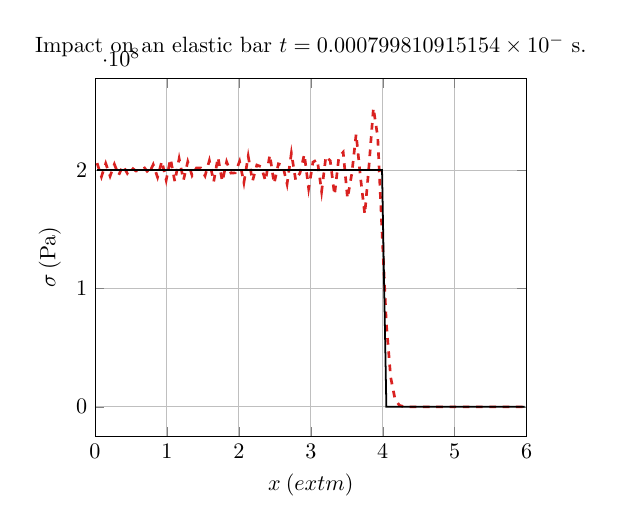
\begin{tikzpicture}[scale=0.8]
\begin{axis}[xlabel=$x \:(	ext{m})$,ylabel=$\sigma \: (\text{Pa})$,ymajorgrids=true,xmajorgrids=true,legend pos=north east,title={Impact on an elastic bar $t = 0.000799810915154\times 10^{-} $ s.},xmin=0.,xmax=6.]
\addplot[Red,very thick,mark=none,dashed] coordinates {(0.03,205801663.056) (0.09,194290281.751) (0.15,205522777.697) (0.21,194765045.219) (0.27,204837977.189) (0.33,195678091.442) (0.39,203676191.803) (0.45,197108930.16) (0.51,201959433.742) (0.57,199120873.566) (0.63,199655686.067) (0.69,201694558.408) (0.75,196858768.899) (0.81,204636822.218) (0.87,193885732.355) (0.93,207485875.371) (0.99,191355550.934) (1.05,209467570.081) (1.11,190174014.86) (1.17,209596824.204) (1.23,191318150.416) (1.29,207030033.346) (1.35,195337558.33) (1.41,201695732.551) (1.47,201641240.416) (1.53,194995238.094) (1.59,207955179.195) (1.65,189996089.745) (1.71,210691220.744) (1.77,190309615.134) (1.83,206923634.091) (1.89,197336628.108) (1.95,197581719.26) (2.01,207292315.833) (2.07,189260409.493) (2.13,211645523.176) (2.19,190620227.071) (2.25,204159086.571) (2.31,202759432.237) (2.37,190781202.887) (2.43,212737259.382) (2.49,188539123.622) (2.55,205205038.908) (2.61,203920794.53) (2.67,188137350.176) (2.73,214227015.38) (2.79,191237758.321) (2.85,197494692.379) (2.91,213192542.634) (2.97,184316952.507) (3.03,206613598.82) (3.09,208789045.003) (3.15,181765168.625) (3.21,211580666.909) (3.27,207740068.787) (3.33,178912332.687) (3.39,211007360.485) (3.45,215043311.113) (3.51,176025142.03) (3.57,196982494.169) (3.63,230309195.474) (3.69,194026599.565) (3.75,162620019.573) (3.81,204636500.028) (3.87,252350248.388) (3.93,227862374.619) (3.99,147549341.154) (4.05,70149900.687) (4.11,24899585.1034) (4.17,6624083.17904) (4.23,1307844.57053) (4.29,186564.480988) (4.35,18224.962181) (4.41,1093.2540344) (4.47,30.4203286797) (4.53,0.0) (4.59,0.0) (4.65,0.0) (4.71,0.0) (4.77,0.0) (4.83,0.0) (4.89,0.0) (4.95,0.0) (5.01,0.0) (5.07,0.0) (5.13,0.0) (5.19,0.0) (5.25,0.0) (5.31,0.0) (5.37,0.0) (5.43,0.0) (5.49,0.0) (5.55,0.0) (5.61,0.0) (5.67,0.0) (5.73,0.0) (5.79,0.0) (5.85,0.0) (5.91,0.0) (5.97,0.0) };
\addplot[black,thick,mark=none,solid] coordinates {(0.03,200000000.0) (0.09,200000000.0) (0.15,200000000.0) (0.21,200000000.0) (0.27,200000000.0) (0.33,200000000.0) (0.39,200000000.0) (0.45,200000000.0) (0.51,200000000.0) (0.57,200000000.0) (0.63,200000000.0) (0.69,200000000.0) (0.75,200000000.0) (0.81,200000000.0) (0.87,200000000.0) (0.93,200000000.0) (0.99,200000000.0) (1.05,200000000.0) (1.11,200000000.0) (1.17,200000000.0) (1.23,200000000.0) (1.29,200000000.0) (1.35,200000000.0) (1.41,200000000.0) (1.47,200000000.0) (1.53,200000000.0) (1.59,200000000.0) (1.65,200000000.0) (1.71,200000000.0) (1.77,200000000.0) (1.83,200000000.0) (1.89,200000000.0) (1.95,200000000.0) (2.01,200000000.0) (2.07,200000000.0) (2.13,200000000.0) (2.19,200000000.0) (2.25,200000000.0) (2.31,200000000.0) (2.37,200000000.0) (2.43,200000000.0) (2.49,200000000.0) (2.55,200000000.0) (2.61,200000000.0) (2.67,200000000.0) (2.73,200000000.0) (2.79,200000000.0) (2.85,200000000.0) (2.91,200000000.0) (2.97,200000000.0) (3.03,200000000.0) (3.09,200000000.0) (3.15,200000000.0) (3.21,200000000.0) (3.27,200000000.0) (3.33,200000000.0) (3.39,200000000.0) (3.45,200000000.0) (3.51,200000000.0) (3.57,200000000.0) (3.63,200000000.0) (3.69,200000000.0) (3.75,200000000.0) (3.81,200000000.0) (3.87,200000000.0) (3.93,200000000.0) (3.99,200000000.0) (4.05,0.0) (4.11,0.0) (4.17,0.0) (4.23,0.0) (4.29,0.0) (4.35,0.0) (4.41,0.0) (4.47,0.0) (4.53,0.0) (4.59,0.0) (4.65,0.0) (4.71,0.0) (4.77,0.0) (4.83,0.0) (4.89,0.0) (4.95,0.0) (5.01,0.0) (5.07,0.0) (5.13,0.0) (5.19,0.0) (5.25,0.0) (5.31,0.0) (5.37,0.0) (5.43,0.0) (5.49,0.0) (5.55,0.0) (5.61,0.0) (5.67,0.0) (5.73,0.0) (5.79,0.0) (5.85,0.0) (5.91,0.0) (5.97,0.0) };
%\legend{fem,exact}
\end{axis}
\end{tikzpicture}
%%% Local Variables:
%%% mode: latex
%%% TeX-master: "../../mainManuscript"
%%% End:

          \end{block}
        \end{column}
      \end{columns}
      \vspace{-0.25cm}
      \footnoteCite{Belytschko}
      \onslide<2>
      %\vspace{-0.58cm}
      \begin{columns}
        \begin{column}{0.49\textwidth}
          \vspace{-0.1cm}
          \begin{block}{The Finite Element Method \cite{Belytschko}}
            \begin{footnotesize}
              \begin{block}{\footnotesize Pros}
                \vspace{-0.2cm}
                \begin{itemize}
                \item[] Non-linear constitutive equations
                \item[] High-order approximation 
                \end{itemize}
              \end{block}
              \vspace{-0.2cm}
              \begin{block}{\footnotesize Cons}
                \vspace{-0.2cm}
                \begin{itemize}
                \item[] Oscillations near discontinuities
                % \item[] Lagrangian: mesh entanglement 
                % \item[] Eulerian: diffusion
                \end{itemize}
              \end{block}
            \end{footnotesize}
          \end{block}
          % \begin{block}{}
          %   \centering
          % % \begin{tikzpicture}[scale=0.4]
% \begin{groupplot}[group style={group size=1 by 1,
% ylabels at=edge left, yticklabels at=edge left,horizontal sep=2.ex,
% vertical sep=4ex,xticklabels at=edge bottom,xlabels at=edge bottom},
% ymajorgrids=true,xmajorgrids=true,enlargelimits=0,xmin=0.,xmax=6.,xlabel=$x (m)$,
% axis on top,scale only axis
% ]
% % \nextgroupplot[ylabel=$\sigma (Pa)$,title={$t = 4.17\times 10^{-4} $ s.},ymin=-1.35e9,ymax=56579516.10614197,]
% % \addplot[Blue,solid,mark=x,very thick,mark size=3pt,mark repeat=3] coordinates{(0.0,-3.2561158711216654e-07) (0.12244897959183673,-6.54162606232603e-22) (0.24489795918367346,0.0) (0.36734693877551017,3.2561158711216643e-07) (0.4897959183673469,-4.884173806682499e-07) (0.6122448979591837,-706703995.0062007) (0.7346938775510203,-739923853.3127105) (0.8571428571428571,-818114621.3278772) (0.9795918367346939,-934350667.0858994) (1.1020408163265305,-1056745717.4113452) (1.2244897959183674,-1153785079.176232) (1.346938775510204,-1213891661.9862223) (1.4693877551020407,-1243675875.166416) (1.5918367346938775,-1255667377.4619899) (1.7142857142857142,-1259628756.7765899) (1.836734693877551,-1260708382.472525) (1.9591836734693877,-1260951555.06527) (2.0816326530612246,-1260996741.6987677) (2.204081632653061,-1261003631.246593) (2.326530612244898,-1261004484.7294881) (2.4489795918367347,-1261004569.3136225) (2.571428571428571,-1261004575.8625927) (2.693877551020408,-1261004576.2443771) (2.816326530612245,-1261004576.2601426) (2.9387755102040813,-1261004576.2605536) (3.061224489795918,-1261004576.2605536) (3.183673469387755,-1261004576.2601426) (3.306122448979592,-1261004576.2443776) (3.4285714285714284,-1261004575.862593) (3.5510204081632653,-1261004569.3136227) (3.673469387755102,-1261004484.7294881) (3.7959183673469385,-1261003631.2465928) (3.9183673469387754,-1260996741.6987677) (4.040816326530612,-1260951555.0652697) (4.163265306122449,-1260708382.4725246) (4.285714285714286,-1259628756.7765894) (4.408163265306122,-1255667377.4619899) (4.530612244897959,-1243675875.1664157) (4.653061224489796,-1213891661.9862223) (4.775510204081632,-1153785079.176232) (4.8979591836734695,-1056745717.4113454) (5.020408163265306,-934350667.0858992) (5.142857142857142,-818114621.327877) (5.26530612244898,-739923853.3127109) (5.387755102040816,-706703995.0062011) (5.5102040816326525,-4.884173806682498e-07) (5.63265306122449,0.0) (5.755102040816326,-4.884173806682498e-07) (5.877551020408163,0.0) (6.0,-4.884173806682498e-07) };
% % \addplot[Purple,solid,mark=+,thick,mark size=3pt,mark repeat=3] coordinates{(0.0,-3.2561158711216654e-07) (0.12244897959183673,-6.54162606232603e-22) (0.24489795918367346,0.0) (0.36734693877551017,3.2561158711216643e-07) (0.4897959183673469,-4.884173806682499e-07) (0.6122448979591837,-710637837.2357953) (0.7346938775510203,-747893724.781927) (0.8571428571428571,-827829409.8631966) (0.9795918367346939,-936780409.853217) (1.1020408163265305,-1054073198.2499647) (1.2244897959183674,-1144128439.1849532) (1.346938775510204,-1207925723.6670742) (1.4693877551020407,-1232372577.7948787) (1.5918367346938775,-1254253728.274747) (1.7142857142857142,-1243570946.3490026) (1.836734693877551,-1268139963.2569304) (1.9591836734693877,-1248035262.8872383) (2.0816326530612246,-1268992337.693115) (2.204081632653061,-1251285653.8729925) (2.326530612244898,-1266352346.5241969) (2.4489795918367347,-1253527311.8706975) (2.571428571428571,-1264419055.233534) (2.693877551020408,-1255474245.0991223) (2.816326530612245,-1261578869.0693417) (2.9387755102040813,-1258168698.6750736) (3.061224489795918,-1258168698.6750731) (3.183673469387755,-1261578869.069342) (3.306122448979592,-1255474245.0991209) (3.4285714285714284,-1264419055.233534) (3.5510204081632653,-1253527311.870696) (3.673469387755102,-1266352346.5241973) (3.7959183673469385,-1251285653.8729923) (3.9183673469387754,-1268992337.6931143) (4.040816326530612,-1248035262.8872375) (4.163265306122449,-1268139963.2569308) (4.285714285714286,-1243570946.3490026) (4.408163265306122,-1254253728.2747467) (4.530612244897959,-1232372577.7948787) (4.653061224489796,-1207925723.6670735) (4.775510204081632,-1144128439.1849532) (4.8979591836734695,-1054073198.2499645) (5.020408163265306,-936780409.853217) (5.142857142857142,-827829409.8631967) (5.26530612244898,-747893724.7819276) (5.387755102040816,-710637837.2357956) (5.5102040816326525,-4.884173806682498e-07) (5.63265306122449,0.0) (5.755102040816326,-4.884173806682498e-07) (5.877551020408163,0.0) (6.0,-4.884173806682498e-07) };
% % \addplot[black,solid,mark=none,thin,mark size=3pt,mark repeat=3] coordinates{(0.0,-0.0) (0.12244897959183673,-0.0) (0.24489795918367346,-0.0) (0.36734693877551017,-0.0) (0.4897959183673469,-0.0) (0.6122448979591837,-700000000.0) (0.7346938775510203,-700000000.0) (0.8571428571428571,-700000000.0) (0.9795918367346939,-700000000.0) (1.1020408163265305,-1261004576.260559) (1.2244897959183674,-1261004576.260559) (1.346938775510204,-1261004576.260559) (1.4693877551020407,-1261004576.260559) (1.5918367346938775,-1261004576.260559) (1.7142857142857142,-1261004576.260559) (1.836734693877551,-1261004576.260559) (1.9591836734693877,-1261004576.260559) (2.0816326530612246,-1261004576.260559) (2.204081632653061,-1261004576.260559) (2.326530612244898,-1261004576.260559) (2.4489795918367347,-1261004576.260559) (2.571428571428571,-1261004576.260559) (2.693877551020408,-1261004576.260559) (2.816326530612245,-1261004576.260559) (2.9387755102040813,-1261004576.260559) (3.061224489795918,-1261004576.260559) (3.183673469387755,-1261004576.260559) (3.306122448979592,-1261004576.260559) (3.4285714285714284,-1261004576.260559) (3.5510204081632653,-1261004576.260559) (3.673469387755102,-1261004576.260559) (3.7959183673469385,-1261004576.260559) (3.9183673469387754,-1261004576.260559) (4.040816326530612,-1261004576.260559) (4.163265306122449,-1261004576.260559) (4.285714285714286,-1261004576.260559) (4.408163265306122,-1261004576.260559) (4.530612244897959,-1261004576.260559) (4.653061224489796,-1261004576.260559) (4.775510204081632,-1261004576.260559) (4.8979591836734695,-1261004576.260559) (5.020408163265306,-700000000.0) (5.142857142857142,-700000000.0) (5.26530612244898,-700000000.0) (5.387755102040816,-700000000.0) (5.5102040816326525,-0.0) (5.63265306122449,-0.0) (5.755102040816326,-0.0) (5.877551020408163,-0.0) (6.0,-0.0) };
% \nextgroupplot[ylabel=$\eps^p $,ymin=-0.0021,ymax=0.0,title={Elastic-plastic plane waves}]
% \addplot[Blue,solid,mark=x,very thick,mark size=3pt,mark repeat=3] coordinates{(0.0,0.0) (0.12244897959183673,0.0) (0.24489795918367346,0.0) (0.36734693877551017,0.0) (0.4897959183673469,0.0) (0.6122448979591837,-2.4267855226065594e-05) (0.7346938775510203,-0.00014452073597361284) (0.8571428571428571,-0.0004275642401009131) (0.9795918367346939,-0.0008483282066457896) (1.1020408163265305,-0.0012913872123487611) (1.2244897959183674,-0.001642660920094959) (1.346938775510204,-0.0018602413103573651) (1.4693877551020407,-0.0019680574666657586) (1.5918367346938775,-0.00201146561977191) (1.7142857142857142,-0.002025805454394895) (1.836734693877551,-0.0020297136017104972) (1.9591836734693877,-0.002030593864489664) (2.0816326530612246,-0.002030757436013639) (2.204081632653061,-0.0020307823755532774) (2.326530612244898,-0.002030785465084119) (2.4489795918367347,-0.0020307857712710334) (2.571428571428571,-0.00203078579497771) (2.693877551020408,-0.0020307857963597366) (2.816326530612245,-0.002030785796416807) (2.9387755102040813,-0.002030785796418294) (3.061224489795918,-0.002030785796418294) (3.183673469387755,-0.0020307857964168056) (3.306122448979592,-0.002030785796359739) (3.4285714285714284,-0.0020307857949777124) (3.5510204081632653,-0.002030785771271032) (3.673469387755102,-0.002030785465084119) (3.7959183673469385,-0.002030782375553277) (3.9183673469387754,-0.0020307574360136386) (4.040816326530612,-0.002030593864489664) (4.163265306122449,-0.0020297136017104964) (4.285714285714286,-0.0020258054543948927) (4.408163265306122,-0.002011465619771909) (4.530612244897959,-0.0019680574666657573) (4.653061224489796,-0.0018602413103573651) (4.775510204081632,-0.0016426609200949592) (4.8979591836734695,-0.001291387212348762) (5.020408163265306,-0.0008483282066457893) (5.142857142857142,-0.00042756424010091193) (5.26530612244898,-0.00014452073597361384) (5.387755102040816,-2.4267855226067292e-05) (5.5102040816326525,0.0) (5.63265306122449,0.0) (5.755102040816326,0.0) (5.877551020408163,0.0) (6.0,0.0) };
% \addplot[Purple,solid,mark=+,thick,mark size=3pt,mark repeat=3] coordinates{(0.0,0.0) (0.12244897959183673,0.0) (0.24489795918367346,0.0) (0.36734693877551017,0.0) (0.4897959183673469,0.0) (0.6122448979591837,-3.850800809337606e-05) (0.7346938775510203,-0.00017337094943683953) (0.8571428571428571,-0.00046273089543238553) (0.9795918367346939,-0.000857123655577256) (1.1020408163265305,-0.0012817129348415013) (1.2244897959183674,-0.0016077047572306) (1.346938775510204,-0.0018386451535459692) (1.4693877551020407,-0.0019271405531036338) (1.5918367346938775,-0.002006348337646142) (1.7142857142857142,-0.002018045326373221) (1.836734693877551,-0.002056615251608797) (1.9591836734693877,-0.0020613216365693464) (2.0816326530612246,-0.002064203896841495) (2.204081632653061,-0.0020644266901542695) (2.326530612244898,-0.0020621094945296272) (2.4489795918367347,-0.002062767607181189) (2.571428571428571,-0.002061489252343496) (2.693877551020408,-0.0020573197208032658) (2.816326530612245,-0.0020502799029179) (2.9387755102040813,-0.0020377776694292327) (3.061224489795918,-0.0020377776694292327) (3.183673469387755,-0.002050279902917899) (3.306122448979592,-0.002057319720803265) (3.4285714285714284,-0.0020614892523434956) (3.5510204081632653,-0.0020627676071811878) (3.673469387755102,-0.0020621094945296285) (3.7959183673469385,-0.0020644266901542695) (3.9183673469387754,-0.0020642038968414953) (4.040816326530612,-0.0020613216365693477) (4.163265306122449,-0.002056615251608799) (4.285714285714286,-0.0020180453263732205) (4.408163265306122,-0.0020063483376461405) (4.530612244897959,-0.0019271405531036334) (4.653061224489796,-0.0018386451535459673) (4.775510204081632,-0.0016077047572305996) (4.8979591836734695,-0.0012817129348415002) (5.020408163265306,-0.0008571236555772557) (5.142857142857142,-0.000462730895432386) (5.26530612244898,-0.0001733709494368422) (5.387755102040816,-3.850800809337776e-05) (5.5102040816326525,0.0) (5.63265306122449,0.0) (5.755102040816326,0.0) (5.877551020408163,0.0) (6.0,0.0) };
% \addplot[black,solid,mark=none,thin,mark size=3pt,mark repeat=3] coordinates{(0.0,-0.0) (0.12244897959183673,-0.0) (0.24489795918367346,-0.0) (0.36734693877551017,-0.0) (0.4897959183673469,-0.0) (0.6122448979591837,-0.0) (0.7346938775510203,-0.0) (0.8571428571428571,-0.0) (0.9795918367346939,-0.0) (1.1020408163265305,-0.002030785796418313) (1.2244897959183674,-0.002030785796418313) (1.346938775510204,-0.002030785796418313) (1.4693877551020407,-0.002030785796418313) (1.5918367346938775,-0.002030785796418313) (1.7142857142857142,-0.002030785796418313) (1.836734693877551,-0.002030785796418313) (1.9591836734693877,-0.002030785796418313) (2.0816326530612246,-0.002030785796418313) (2.204081632653061,-0.002030785796418313) (2.326530612244898,-0.002030785796418313) (2.4489795918367347,-0.002030785796418313) (2.571428571428571,-0.002030785796418313) (2.693877551020408,-0.002030785796418313) (2.816326530612245,-0.002030785796418313) (2.9387755102040813,-0.002030785796418313) (3.061224489795918,-0.002030785796418313) (3.183673469387755,-0.002030785796418313) (3.306122448979592,-0.002030785796418313) (3.4285714285714284,-0.002030785796418313) (3.5510204081632653,-0.002030785796418313) (3.673469387755102,-0.002030785796418313) (3.7959183673469385,-0.002030785796418313) (3.9183673469387754,-0.002030785796418313) (4.040816326530612,-0.002030785796418313) (4.163265306122449,-0.002030785796418313) (4.285714285714286,-0.002030785796418313) (4.408163265306122,-0.002030785796418313) (4.530612244897959,-0.002030785796418313) (4.653061224489796,-0.002030785796418313) (4.775510204081632,-0.002030785796418313) (4.8979591836734695,-0.002030785796418313) (5.020408163265306,-0.0) (5.142857142857142,-0.0) (5.26530612244898,-0.0) (5.387755102040816,-0.0) (5.5102040816326525,-0.0) (5.63265306122449,-0.0) (5.755102040816326,-0.0) (5.877551020408163,-0.0) (6.0,-0.0) };

% \addlegendentry{fvm (elastic-plastic Riemann solver)}
% \addlegendentry{fvm (elastic Riemann solver)}
% \addlegendentry{exact}

% \end{groupplot}
% \end{tikzpicture}


\begin{tikzpicture}[spy using outlines={rectangle, magnification=2, size=.15cm, connect spies},scale=0.6]
\begin{axis}[xlabel=$x \:(\text{m})$,ylabel=$\eps^p $,ymajorgrids=true,xmajorgrids=true,legend pos=north east,title={Plastic waves},xmin=0.,xmax=6.,ymin=-0.0021,ymax=0.00001]
\addplot[Blue,solid,mark=x,very thick,mark size=3pt,mark repeat=3] coordinates{(0.0,0.0) (0.12244897959183673,0.0) (0.24489795918367346,0.0) (0.36734693877551017,0.0) (0.4897959183673469,0.0) (0.6122448979591837,-2.4267855226065594e-05) (0.7346938775510203,-0.00014452073597361284) (0.8571428571428571,-0.0004275642401009131) (0.9795918367346939,-0.0008483282066457896) (1.1020408163265305,-0.0012913872123487611) (1.2244897959183674,-0.001642660920094959) (1.346938775510204,-0.0018602413103573651) (1.4693877551020407,-0.0019680574666657586) (1.5918367346938775,-0.00201146561977191) (1.7142857142857142,-0.002025805454394895) (1.836734693877551,-0.0020297136017104972) (1.9591836734693877,-0.002030593864489664) (2.0816326530612246,-0.002030757436013639) (2.204081632653061,-0.0020307823755532774) (2.326530612244898,-0.002030785465084119) (2.4489795918367347,-0.0020307857712710334) (2.571428571428571,-0.00203078579497771) (2.693877551020408,-0.0020307857963597366) (2.816326530612245,-0.002030785796416807) (2.9387755102040813,-0.002030785796418294) (3.061224489795918,-0.002030785796418294) (3.183673469387755,-0.0020307857964168056) (3.306122448979592,-0.002030785796359739) (3.4285714285714284,-0.0020307857949777124) (3.5510204081632653,-0.002030785771271032) (3.673469387755102,-0.002030785465084119) (3.7959183673469385,-0.002030782375553277) (3.9183673469387754,-0.0020307574360136386) (4.040816326530612,-0.002030593864489664) (4.163265306122449,-0.0020297136017104964) (4.285714285714286,-0.0020258054543948927) (4.408163265306122,-0.002011465619771909) (4.530612244897959,-0.0019680574666657573) (4.653061224489796,-0.0018602413103573651) (4.775510204081632,-0.0016426609200949592) (4.8979591836734695,-0.001291387212348762) (5.020408163265306,-0.0008483282066457893) (5.142857142857142,-0.00042756424010091193) (5.26530612244898,-0.00014452073597361384) (5.387755102040816,-2.4267855226067292e-05) (5.5102040816326525,0.0) (5.63265306122449,0.0) (5.755102040816326,0.0) (5.877551020408163,0.0) (6.0,0.0) };
\addplot[Red,solid,mark=+,very thick,mark size=3pt,mark repeat=3] coordinates{(0.0,0.0) (0.12244897959183673,0.0) (0.24489795918367346,0.0) (0.36734693877551017,0.0) (0.4897959183673469,0.0) (0.6122448979591837,-3.850800809337606e-05) (0.7346938775510203,-0.00017337094943683953) (0.8571428571428571,-0.00046273089543238553) (0.9795918367346939,-0.000857123655577256) (1.1020408163265305,-0.0012817129348415013) (1.2244897959183674,-0.0016077047572306) (1.346938775510204,-0.0018386451535459692) (1.4693877551020407,-0.0019271405531036338) (1.5918367346938775,-0.002006348337646142) (1.7142857142857142,-0.002018045326373221) (1.836734693877551,-0.002056615251608797) (1.9591836734693877,-0.0020613216365693464) (2.0816326530612246,-0.002064203896841495) (2.204081632653061,-0.0020644266901542695) (2.326530612244898,-0.0020621094945296272) (2.4489795918367347,-0.002062767607181189) (2.571428571428571,-0.002061489252343496) (2.693877551020408,-0.0020573197208032658) (2.816326530612245,-0.0020502799029179) (2.9387755102040813,-0.0020377776694292327) (3.061224489795918,-0.0020377776694292327) (3.183673469387755,-0.002050279902917899) (3.306122448979592,-0.002057319720803265) (3.4285714285714284,-0.0020614892523434956) (3.5510204081632653,-0.0020627676071811878) (3.673469387755102,-0.0020621094945296285) (3.7959183673469385,-0.0020644266901542695) (3.9183673469387754,-0.0020642038968414953) (4.040816326530612,-0.0020613216365693477) (4.163265306122449,-0.002056615251608799) (4.285714285714286,-0.0020180453263732205) (4.408163265306122,-0.0020063483376461405) (4.530612244897959,-0.0019271405531036334) (4.653061224489796,-0.0018386451535459673) (4.775510204081632,-0.0016077047572305996) (4.8979591836734695,-0.0012817129348415002) (5.020408163265306,-0.0008571236555772557) (5.142857142857142,-0.000462730895432386) (5.26530612244898,-0.0001733709494368422) (5.387755102040816,-3.850800809337776e-05) (5.5102040816326525,0.0) (5.63265306122449,0.0) (5.755102040816326,0.0) (5.877551020408163,0.0) (6.0,0.0) };
\addplot[black,solid,mark=none,thick,mark size=3pt,mark repeat=3] coordinates{(0.0,-0.0) (0.12244897959183673,-0.0) (0.24489795918367346,-0.0) (0.36734693877551017,-0.0) (0.4897959183673469,-0.0) (0.6122448979591837,-0.0) (0.7346938775510203,-0.0) (0.8571428571428571,-0.0) (0.9795918367346939,-0.0) (1.1020408163265305,-0.002030785796418313) (1.2244897959183674,-0.002030785796418313) (1.346938775510204,-0.002030785796418313) (1.4693877551020407,-0.002030785796418313) (1.5918367346938775,-0.002030785796418313) (1.7142857142857142,-0.002030785796418313) (1.836734693877551,-0.002030785796418313) (1.9591836734693877,-0.002030785796418313) (2.0816326530612246,-0.002030785796418313) (2.204081632653061,-0.002030785796418313) (2.326530612244898,-0.002030785796418313) (2.4489795918367347,-0.002030785796418313) (2.571428571428571,-0.002030785796418313) (2.693877551020408,-0.002030785796418313) (2.816326530612245,-0.002030785796418313) (2.9387755102040813,-0.002030785796418313) (3.061224489795918,-0.002030785796418313) (3.183673469387755,-0.002030785796418313) (3.306122448979592,-0.002030785796418313) (3.4285714285714284,-0.002030785796418313) (3.5510204081632653,-0.002030785796418313) (3.673469387755102,-0.002030785796418313) (3.7959183673469385,-0.002030785796418313) (3.9183673469387754,-0.002030785796418313) (4.040816326530612,-0.002030785796418313) (4.163265306122449,-0.002030785796418313) (4.285714285714286,-0.002030785796418313) (4.408163265306122,-0.002030785796418313) (4.530612244897959,-0.002030785796418313) (4.653061224489796,-0.002030785796418313) (4.775510204081632,-0.002030785796418313) (4.8979591836734695,-0.002030785796418313) (5.020408163265306,-0.0) (5.142857142857142,-0.0) (5.26530612244898,-0.0) (5.387755102040816,-0.0) (5.5102040816326525,-0.0) (5.63265306122449,-0.0) (5.755102040816326,-0.0) (5.877551020408163,-0.0) (6.0,-0.0) };
\begin{scope}
\spy[black,size=1.5cm] on (1.25,0.3) in node [fill=none] at (3.5,2.7);
\end{scope}

\legend{fvm ("elastic" fluxes),fvm ("elastic-plastic" fluxes),exact}
\end{axis}
\end{tikzpicture}
%%% Local Variables:
%%% mode: latex
%%% TeX-master: "../../presentation"
%%% End:

          % \end{block}
          
        \end{column}
        \begin{column}{0.49\textwidth}
          \begin{block}{The Finite Volume Method \cite{Leveque}}
            \begin{footnotesize}
              \begin{block}{\footnotesize Pros}
                \vspace{-0.2cm}
                \begin{itemize}
                \item[] Conservation laws % donc même approx de v et F + bien pour estimer la vitesse des chocs
                \item[] Use of numerical fluxes \cite{Godunov_method}
                \end{itemize}
              \end{block}
              \vspace{-0.2cm}
              \begin{block}{\footnotesize Cons}
                \vspace{-0.2cm}
                \begin{itemize}
                \item[] Essentially low-order methods
                % \item[] Lagrangian \cite{Haider_FVM}: update geometries  
                % \item[] Eulerian \cite{Gavrilyuk}: constitutive equations ?
                \end{itemize}
              \end{block}
            \end{footnotesize}
          \end{block}
        \end{column}
      \end{columns}
      \vspace{-0.3cm} 
      \footnoteCite{Leveque,Godunov_method,Thomas_EP}
      
      \onslide<3>
      \begin{columns}
        \begin{column}{0.49\textwidth}
          \vspace{-0.1cm}
          \begin{block}{The Finite Element Method \cite{Belytschko}}
            \begin{footnotesize}
              \begin{block}{\footnotesize Pros}
                \vspace{-0.2cm}
                \begin{itemize}
                \item[] Non-linear constitutive equations
                \item[] High-order approximation 
                \end{itemize}
              \end{block}
              \vspace{-0.2cm}
              \begin{block}{\footnotesize Cons}
                \vspace{-0.2cm}
                \begin{itemize}
                \item[] Oscillations
                \item[] Lagrangian: mesh-difficulties% entanglement 
                \item[] Eulerian: numerical diffusion %--tracking of interfaces
                \end{itemize}
              \end{block}
            \end{footnotesize}
          \end{block}
        \end{column}
        \begin{column}{0.49\textwidth}
          \begin{block}{The Finite Volume Method \cite{Leveque}}
            \begin{footnotesize}
              \begin{block}{\footnotesize Pros}
                \vspace{-0.2cm}
                \begin{itemize}
                \item[] Conservation laws % donc même approx de v et F
                \item[] Use of numerical fluxes \cite{Godunov_method}
                \end{itemize}
              \end{block}
              \vspace{-0.2cm}
              \begin{block}{\footnotesize Cons}
                \vspace{-0.2cm}
                \begin{itemize}
                \item[] Essentially low-order methods
                \item[] Lagrangian \cite{Haider_FVM}: mesh-difficulties %update geometries  
                \item[] Eulerian \cite{Gavrilyuk}: numerical diffusion%--tracking of interfaces
                \end{itemize}
              \end{block}
            \end{footnotesize}
          \end{block}
        \end{column}
      \end{columns}
      
      \vspace{-0.3cm} 
      \footnoteCite{Belytschko,Leveque,Godunov_method,Haider_FVM,Gavrilyuk}
    \end{overprint}
  \end{frame}
\end{withoutheadline}

\begin{withoutheadline}
  \begin{frame}{Some explicit numerical methods}
    \begin{block}{The space-Discontinuous Galerkin Finite Element Method \cite{Cockburn}}
      \begin{footnotesize}
        \begin{block}{\footnotesize Merge FVM and FEM}
          \vspace{-.2cm}
          \begin{itemize}
          \item[] Local high-order approximation \cite{NeutronDG}
          \item[] Same approximation of field and gradient
          \item[] Numerical fluxes: no oscillations
          \end{itemize}
        \end{block}
        \vspace{-.2cm}
        \begin{block}{\footnotesize Limitations}
          \vspace{-.2cm}
          \begin{itemize}
          \item[] Restrictive time step
          \item[] Lagrangian: update of the geometry \cite{LagrangianDG_thesis}
          \item[] Eulerian: numerical diffusion -- interface tracking%diffusive advection terms -- constitutive equaions
          \end{itemize}
        \end{block}
      \end{footnotesize}
    \end{block}
    \footnoteCite{Cockburn,NeutronDG,LagrangianDG_thesis}
  \end{frame}
\end{withoutheadline}


\begin{withoutheadline}
  \begin{frame}{Mesh-free Lagrangian approaches}
    
    \begin{block}{The Material Point Method \cite{Sulsky94}}
      \begin{footnotesize}
        \begin{itemize}
        \item Particle-based space discretization
        \item Arbitrary computational grid
        \end{itemize}
      \end{footnotesize}
      
      \centering
      \textbf{Projections of fields Particles $\leftrightarrow$ Nodes}
    \end{block}

    \begin{columns}
      \begin{column}{0.48\textwidth}
        \begin{block}{\footnotesize Particle-In-Cell mapping \cite{PIC}}
          \begin{footnotesize}
            \begin{itemize}
            \item[] No oscillations 
            \item[] Numerical diffusion
            \end{itemize}
          \end{footnotesize}
        \end{block}
      \end{column}
      \begin{column}{0.48\textwidth}
        \begin{block}{\footnotesize FLuid Implicit Particle mapping \cite{PIC_Nishiguchi}}
          \begin{footnotesize}
            \begin{itemize}
            \item[] Reduced diffusion 
            \item[] Oscillations
            \end{itemize}
          \end{footnotesize}
        \end{block}
      \end{column}
    \end{columns}
    \vspace{-0.3cm}
    \footnoteCite{Sulsky94,PIC,PIC_Nishiguchi}
  \end{frame}
\end{withoutheadline}

\begin{withoutheadline}
  \begin{frame}{\text{  }}
    \vspace{-0.4cm}
    \begin{overprint}
      \onslide<1>
      \begin{block}{Challenging task for numerical methods}
        \alert{Accurately track waves in finite deforming elastic-plastic solids}
        \begin{itemize}
          \item[]
          % \item[1-] Handle large deformations -- No oscillation -- Low diffusion
        \item[]
          % \item[2-] Embed sufficient amount of information about the solution (intercell fluxes)
        \end{itemize}
      \end{block}
      \onslide<2>
      \begin{block}{Challenging task for numerical methods}
        \alert{Accurately track waves in finite deforming elastic-plastic solids}
        \begin{itemize}
        \item[1-] \textbf{Handle large deformations -- No oscillation -- Low diffusion}
          \item[]
        %\item[2-] Embed sufficient amount of information about the solution (intercell fluxes)
        \end{itemize}
      \end{block}
      \metroset{block=fill}
      \begin{block}{Objective 1}
        Develop a numerical method that accurately capture waves in finite deforming solids \\
        \textbf{Merge FEM--FVM--MPM: DG approximation}
      \end{block}
      \onslide<3>
      \begin{block}{Challenging task for numerical methods}
        \alert{Accurately track waves in finite deforming elastic-plastic solids}
        \begin{itemize}
        \item[1-] Handle large deformations -- No oscillation -- Low diffusion
        \item[2-] \textbf{Embed sufficient amount of information about the solution (intercell fluxes \cite{Thomas_EP})}
        \end{itemize}
      \end{block}
      \vspace{-0.9cm}
      \begin{block}{}
        \centering
        % \begin{tikzpicture}[scale=0.4]
% \begin{groupplot}[group style={group size=1 by 1,
% ylabels at=edge left, yticklabels at=edge left,horizontal sep=2.ex,
% vertical sep=4ex,xticklabels at=edge bottom,xlabels at=edge bottom},
% ymajorgrids=true,xmajorgrids=true,enlargelimits=0,xmin=0.,xmax=6.,xlabel=$x (m)$,
% axis on top,scale only axis
% ]
% % \nextgroupplot[ylabel=$\sigma (Pa)$,title={$t = 4.17\times 10^{-4} $ s.},ymin=-1.35e9,ymax=56579516.10614197,]
% % \addplot[Blue,solid,mark=x,very thick,mark size=3pt,mark repeat=3] coordinates{(0.0,-3.2561158711216654e-07) (0.12244897959183673,-6.54162606232603e-22) (0.24489795918367346,0.0) (0.36734693877551017,3.2561158711216643e-07) (0.4897959183673469,-4.884173806682499e-07) (0.6122448979591837,-706703995.0062007) (0.7346938775510203,-739923853.3127105) (0.8571428571428571,-818114621.3278772) (0.9795918367346939,-934350667.0858994) (1.1020408163265305,-1056745717.4113452) (1.2244897959183674,-1153785079.176232) (1.346938775510204,-1213891661.9862223) (1.4693877551020407,-1243675875.166416) (1.5918367346938775,-1255667377.4619899) (1.7142857142857142,-1259628756.7765899) (1.836734693877551,-1260708382.472525) (1.9591836734693877,-1260951555.06527) (2.0816326530612246,-1260996741.6987677) (2.204081632653061,-1261003631.246593) (2.326530612244898,-1261004484.7294881) (2.4489795918367347,-1261004569.3136225) (2.571428571428571,-1261004575.8625927) (2.693877551020408,-1261004576.2443771) (2.816326530612245,-1261004576.2601426) (2.9387755102040813,-1261004576.2605536) (3.061224489795918,-1261004576.2605536) (3.183673469387755,-1261004576.2601426) (3.306122448979592,-1261004576.2443776) (3.4285714285714284,-1261004575.862593) (3.5510204081632653,-1261004569.3136227) (3.673469387755102,-1261004484.7294881) (3.7959183673469385,-1261003631.2465928) (3.9183673469387754,-1260996741.6987677) (4.040816326530612,-1260951555.0652697) (4.163265306122449,-1260708382.4725246) (4.285714285714286,-1259628756.7765894) (4.408163265306122,-1255667377.4619899) (4.530612244897959,-1243675875.1664157) (4.653061224489796,-1213891661.9862223) (4.775510204081632,-1153785079.176232) (4.8979591836734695,-1056745717.4113454) (5.020408163265306,-934350667.0858992) (5.142857142857142,-818114621.327877) (5.26530612244898,-739923853.3127109) (5.387755102040816,-706703995.0062011) (5.5102040816326525,-4.884173806682498e-07) (5.63265306122449,0.0) (5.755102040816326,-4.884173806682498e-07) (5.877551020408163,0.0) (6.0,-4.884173806682498e-07) };
% % \addplot[Purple,solid,mark=+,thick,mark size=3pt,mark repeat=3] coordinates{(0.0,-3.2561158711216654e-07) (0.12244897959183673,-6.54162606232603e-22) (0.24489795918367346,0.0) (0.36734693877551017,3.2561158711216643e-07) (0.4897959183673469,-4.884173806682499e-07) (0.6122448979591837,-710637837.2357953) (0.7346938775510203,-747893724.781927) (0.8571428571428571,-827829409.8631966) (0.9795918367346939,-936780409.853217) (1.1020408163265305,-1054073198.2499647) (1.2244897959183674,-1144128439.1849532) (1.346938775510204,-1207925723.6670742) (1.4693877551020407,-1232372577.7948787) (1.5918367346938775,-1254253728.274747) (1.7142857142857142,-1243570946.3490026) (1.836734693877551,-1268139963.2569304) (1.9591836734693877,-1248035262.8872383) (2.0816326530612246,-1268992337.693115) (2.204081632653061,-1251285653.8729925) (2.326530612244898,-1266352346.5241969) (2.4489795918367347,-1253527311.8706975) (2.571428571428571,-1264419055.233534) (2.693877551020408,-1255474245.0991223) (2.816326530612245,-1261578869.0693417) (2.9387755102040813,-1258168698.6750736) (3.061224489795918,-1258168698.6750731) (3.183673469387755,-1261578869.069342) (3.306122448979592,-1255474245.0991209) (3.4285714285714284,-1264419055.233534) (3.5510204081632653,-1253527311.870696) (3.673469387755102,-1266352346.5241973) (3.7959183673469385,-1251285653.8729923) (3.9183673469387754,-1268992337.6931143) (4.040816326530612,-1248035262.8872375) (4.163265306122449,-1268139963.2569308) (4.285714285714286,-1243570946.3490026) (4.408163265306122,-1254253728.2747467) (4.530612244897959,-1232372577.7948787) (4.653061224489796,-1207925723.6670735) (4.775510204081632,-1144128439.1849532) (4.8979591836734695,-1054073198.2499645) (5.020408163265306,-936780409.853217) (5.142857142857142,-827829409.8631967) (5.26530612244898,-747893724.7819276) (5.387755102040816,-710637837.2357956) (5.5102040816326525,-4.884173806682498e-07) (5.63265306122449,0.0) (5.755102040816326,-4.884173806682498e-07) (5.877551020408163,0.0) (6.0,-4.884173806682498e-07) };
% % \addplot[black,solid,mark=none,thin,mark size=3pt,mark repeat=3] coordinates{(0.0,-0.0) (0.12244897959183673,-0.0) (0.24489795918367346,-0.0) (0.36734693877551017,-0.0) (0.4897959183673469,-0.0) (0.6122448979591837,-700000000.0) (0.7346938775510203,-700000000.0) (0.8571428571428571,-700000000.0) (0.9795918367346939,-700000000.0) (1.1020408163265305,-1261004576.260559) (1.2244897959183674,-1261004576.260559) (1.346938775510204,-1261004576.260559) (1.4693877551020407,-1261004576.260559) (1.5918367346938775,-1261004576.260559) (1.7142857142857142,-1261004576.260559) (1.836734693877551,-1261004576.260559) (1.9591836734693877,-1261004576.260559) (2.0816326530612246,-1261004576.260559) (2.204081632653061,-1261004576.260559) (2.326530612244898,-1261004576.260559) (2.4489795918367347,-1261004576.260559) (2.571428571428571,-1261004576.260559) (2.693877551020408,-1261004576.260559) (2.816326530612245,-1261004576.260559) (2.9387755102040813,-1261004576.260559) (3.061224489795918,-1261004576.260559) (3.183673469387755,-1261004576.260559) (3.306122448979592,-1261004576.260559) (3.4285714285714284,-1261004576.260559) (3.5510204081632653,-1261004576.260559) (3.673469387755102,-1261004576.260559) (3.7959183673469385,-1261004576.260559) (3.9183673469387754,-1261004576.260559) (4.040816326530612,-1261004576.260559) (4.163265306122449,-1261004576.260559) (4.285714285714286,-1261004576.260559) (4.408163265306122,-1261004576.260559) (4.530612244897959,-1261004576.260559) (4.653061224489796,-1261004576.260559) (4.775510204081632,-1261004576.260559) (4.8979591836734695,-1261004576.260559) (5.020408163265306,-700000000.0) (5.142857142857142,-700000000.0) (5.26530612244898,-700000000.0) (5.387755102040816,-700000000.0) (5.5102040816326525,-0.0) (5.63265306122449,-0.0) (5.755102040816326,-0.0) (5.877551020408163,-0.0) (6.0,-0.0) };
% \nextgroupplot[ylabel=$\eps^p $,ymin=-0.0021,ymax=0.0,title={Elastic-plastic plane waves}]
% \addplot[Blue,solid,mark=x,very thick,mark size=3pt,mark repeat=3] coordinates{(0.0,0.0) (0.12244897959183673,0.0) (0.24489795918367346,0.0) (0.36734693877551017,0.0) (0.4897959183673469,0.0) (0.6122448979591837,-2.4267855226065594e-05) (0.7346938775510203,-0.00014452073597361284) (0.8571428571428571,-0.0004275642401009131) (0.9795918367346939,-0.0008483282066457896) (1.1020408163265305,-0.0012913872123487611) (1.2244897959183674,-0.001642660920094959) (1.346938775510204,-0.0018602413103573651) (1.4693877551020407,-0.0019680574666657586) (1.5918367346938775,-0.00201146561977191) (1.7142857142857142,-0.002025805454394895) (1.836734693877551,-0.0020297136017104972) (1.9591836734693877,-0.002030593864489664) (2.0816326530612246,-0.002030757436013639) (2.204081632653061,-0.0020307823755532774) (2.326530612244898,-0.002030785465084119) (2.4489795918367347,-0.0020307857712710334) (2.571428571428571,-0.00203078579497771) (2.693877551020408,-0.0020307857963597366) (2.816326530612245,-0.002030785796416807) (2.9387755102040813,-0.002030785796418294) (3.061224489795918,-0.002030785796418294) (3.183673469387755,-0.0020307857964168056) (3.306122448979592,-0.002030785796359739) (3.4285714285714284,-0.0020307857949777124) (3.5510204081632653,-0.002030785771271032) (3.673469387755102,-0.002030785465084119) (3.7959183673469385,-0.002030782375553277) (3.9183673469387754,-0.0020307574360136386) (4.040816326530612,-0.002030593864489664) (4.163265306122449,-0.0020297136017104964) (4.285714285714286,-0.0020258054543948927) (4.408163265306122,-0.002011465619771909) (4.530612244897959,-0.0019680574666657573) (4.653061224489796,-0.0018602413103573651) (4.775510204081632,-0.0016426609200949592) (4.8979591836734695,-0.001291387212348762) (5.020408163265306,-0.0008483282066457893) (5.142857142857142,-0.00042756424010091193) (5.26530612244898,-0.00014452073597361384) (5.387755102040816,-2.4267855226067292e-05) (5.5102040816326525,0.0) (5.63265306122449,0.0) (5.755102040816326,0.0) (5.877551020408163,0.0) (6.0,0.0) };
% \addplot[Purple,solid,mark=+,thick,mark size=3pt,mark repeat=3] coordinates{(0.0,0.0) (0.12244897959183673,0.0) (0.24489795918367346,0.0) (0.36734693877551017,0.0) (0.4897959183673469,0.0) (0.6122448979591837,-3.850800809337606e-05) (0.7346938775510203,-0.00017337094943683953) (0.8571428571428571,-0.00046273089543238553) (0.9795918367346939,-0.000857123655577256) (1.1020408163265305,-0.0012817129348415013) (1.2244897959183674,-0.0016077047572306) (1.346938775510204,-0.0018386451535459692) (1.4693877551020407,-0.0019271405531036338) (1.5918367346938775,-0.002006348337646142) (1.7142857142857142,-0.002018045326373221) (1.836734693877551,-0.002056615251608797) (1.9591836734693877,-0.0020613216365693464) (2.0816326530612246,-0.002064203896841495) (2.204081632653061,-0.0020644266901542695) (2.326530612244898,-0.0020621094945296272) (2.4489795918367347,-0.002062767607181189) (2.571428571428571,-0.002061489252343496) (2.693877551020408,-0.0020573197208032658) (2.816326530612245,-0.0020502799029179) (2.9387755102040813,-0.0020377776694292327) (3.061224489795918,-0.0020377776694292327) (3.183673469387755,-0.002050279902917899) (3.306122448979592,-0.002057319720803265) (3.4285714285714284,-0.0020614892523434956) (3.5510204081632653,-0.0020627676071811878) (3.673469387755102,-0.0020621094945296285) (3.7959183673469385,-0.0020644266901542695) (3.9183673469387754,-0.0020642038968414953) (4.040816326530612,-0.0020613216365693477) (4.163265306122449,-0.002056615251608799) (4.285714285714286,-0.0020180453263732205) (4.408163265306122,-0.0020063483376461405) (4.530612244897959,-0.0019271405531036334) (4.653061224489796,-0.0018386451535459673) (4.775510204081632,-0.0016077047572305996) (4.8979591836734695,-0.0012817129348415002) (5.020408163265306,-0.0008571236555772557) (5.142857142857142,-0.000462730895432386) (5.26530612244898,-0.0001733709494368422) (5.387755102040816,-3.850800809337776e-05) (5.5102040816326525,0.0) (5.63265306122449,0.0) (5.755102040816326,0.0) (5.877551020408163,0.0) (6.0,0.0) };
% \addplot[black,solid,mark=none,thin,mark size=3pt,mark repeat=3] coordinates{(0.0,-0.0) (0.12244897959183673,-0.0) (0.24489795918367346,-0.0) (0.36734693877551017,-0.0) (0.4897959183673469,-0.0) (0.6122448979591837,-0.0) (0.7346938775510203,-0.0) (0.8571428571428571,-0.0) (0.9795918367346939,-0.0) (1.1020408163265305,-0.002030785796418313) (1.2244897959183674,-0.002030785796418313) (1.346938775510204,-0.002030785796418313) (1.4693877551020407,-0.002030785796418313) (1.5918367346938775,-0.002030785796418313) (1.7142857142857142,-0.002030785796418313) (1.836734693877551,-0.002030785796418313) (1.9591836734693877,-0.002030785796418313) (2.0816326530612246,-0.002030785796418313) (2.204081632653061,-0.002030785796418313) (2.326530612244898,-0.002030785796418313) (2.4489795918367347,-0.002030785796418313) (2.571428571428571,-0.002030785796418313) (2.693877551020408,-0.002030785796418313) (2.816326530612245,-0.002030785796418313) (2.9387755102040813,-0.002030785796418313) (3.061224489795918,-0.002030785796418313) (3.183673469387755,-0.002030785796418313) (3.306122448979592,-0.002030785796418313) (3.4285714285714284,-0.002030785796418313) (3.5510204081632653,-0.002030785796418313) (3.673469387755102,-0.002030785796418313) (3.7959183673469385,-0.002030785796418313) (3.9183673469387754,-0.002030785796418313) (4.040816326530612,-0.002030785796418313) (4.163265306122449,-0.002030785796418313) (4.285714285714286,-0.002030785796418313) (4.408163265306122,-0.002030785796418313) (4.530612244897959,-0.002030785796418313) (4.653061224489796,-0.002030785796418313) (4.775510204081632,-0.002030785796418313) (4.8979591836734695,-0.002030785796418313) (5.020408163265306,-0.0) (5.142857142857142,-0.0) (5.26530612244898,-0.0) (5.387755102040816,-0.0) (5.5102040816326525,-0.0) (5.63265306122449,-0.0) (5.755102040816326,-0.0) (5.877551020408163,-0.0) (6.0,-0.0) };

% \addlegendentry{fvm (elastic-plastic Riemann solver)}
% \addlegendentry{fvm (elastic Riemann solver)}
% \addlegendentry{exact}

% \end{groupplot}
% \end{tikzpicture}


\begin{tikzpicture}[spy using outlines={rectangle, magnification=2, size=.15cm, connect spies},scale=0.6]
\begin{axis}[xlabel=$x \:(\text{m})$,ylabel=$\eps^p $,ymajorgrids=true,xmajorgrids=true,legend pos=north east,title={Plastic waves},xmin=0.,xmax=6.,ymin=-0.0021,ymax=0.00001]
\addplot[Blue,solid,mark=x,very thick,mark size=3pt,mark repeat=3] coordinates{(0.0,0.0) (0.12244897959183673,0.0) (0.24489795918367346,0.0) (0.36734693877551017,0.0) (0.4897959183673469,0.0) (0.6122448979591837,-2.4267855226065594e-05) (0.7346938775510203,-0.00014452073597361284) (0.8571428571428571,-0.0004275642401009131) (0.9795918367346939,-0.0008483282066457896) (1.1020408163265305,-0.0012913872123487611) (1.2244897959183674,-0.001642660920094959) (1.346938775510204,-0.0018602413103573651) (1.4693877551020407,-0.0019680574666657586) (1.5918367346938775,-0.00201146561977191) (1.7142857142857142,-0.002025805454394895) (1.836734693877551,-0.0020297136017104972) (1.9591836734693877,-0.002030593864489664) (2.0816326530612246,-0.002030757436013639) (2.204081632653061,-0.0020307823755532774) (2.326530612244898,-0.002030785465084119) (2.4489795918367347,-0.0020307857712710334) (2.571428571428571,-0.00203078579497771) (2.693877551020408,-0.0020307857963597366) (2.816326530612245,-0.002030785796416807) (2.9387755102040813,-0.002030785796418294) (3.061224489795918,-0.002030785796418294) (3.183673469387755,-0.0020307857964168056) (3.306122448979592,-0.002030785796359739) (3.4285714285714284,-0.0020307857949777124) (3.5510204081632653,-0.002030785771271032) (3.673469387755102,-0.002030785465084119) (3.7959183673469385,-0.002030782375553277) (3.9183673469387754,-0.0020307574360136386) (4.040816326530612,-0.002030593864489664) (4.163265306122449,-0.0020297136017104964) (4.285714285714286,-0.0020258054543948927) (4.408163265306122,-0.002011465619771909) (4.530612244897959,-0.0019680574666657573) (4.653061224489796,-0.0018602413103573651) (4.775510204081632,-0.0016426609200949592) (4.8979591836734695,-0.001291387212348762) (5.020408163265306,-0.0008483282066457893) (5.142857142857142,-0.00042756424010091193) (5.26530612244898,-0.00014452073597361384) (5.387755102040816,-2.4267855226067292e-05) (5.5102040816326525,0.0) (5.63265306122449,0.0) (5.755102040816326,0.0) (5.877551020408163,0.0) (6.0,0.0) };
\addplot[Red,solid,mark=+,very thick,mark size=3pt,mark repeat=3] coordinates{(0.0,0.0) (0.12244897959183673,0.0) (0.24489795918367346,0.0) (0.36734693877551017,0.0) (0.4897959183673469,0.0) (0.6122448979591837,-3.850800809337606e-05) (0.7346938775510203,-0.00017337094943683953) (0.8571428571428571,-0.00046273089543238553) (0.9795918367346939,-0.000857123655577256) (1.1020408163265305,-0.0012817129348415013) (1.2244897959183674,-0.0016077047572306) (1.346938775510204,-0.0018386451535459692) (1.4693877551020407,-0.0019271405531036338) (1.5918367346938775,-0.002006348337646142) (1.7142857142857142,-0.002018045326373221) (1.836734693877551,-0.002056615251608797) (1.9591836734693877,-0.0020613216365693464) (2.0816326530612246,-0.002064203896841495) (2.204081632653061,-0.0020644266901542695) (2.326530612244898,-0.0020621094945296272) (2.4489795918367347,-0.002062767607181189) (2.571428571428571,-0.002061489252343496) (2.693877551020408,-0.0020573197208032658) (2.816326530612245,-0.0020502799029179) (2.9387755102040813,-0.0020377776694292327) (3.061224489795918,-0.0020377776694292327) (3.183673469387755,-0.002050279902917899) (3.306122448979592,-0.002057319720803265) (3.4285714285714284,-0.0020614892523434956) (3.5510204081632653,-0.0020627676071811878) (3.673469387755102,-0.0020621094945296285) (3.7959183673469385,-0.0020644266901542695) (3.9183673469387754,-0.0020642038968414953) (4.040816326530612,-0.0020613216365693477) (4.163265306122449,-0.002056615251608799) (4.285714285714286,-0.0020180453263732205) (4.408163265306122,-0.0020063483376461405) (4.530612244897959,-0.0019271405531036334) (4.653061224489796,-0.0018386451535459673) (4.775510204081632,-0.0016077047572305996) (4.8979591836734695,-0.0012817129348415002) (5.020408163265306,-0.0008571236555772557) (5.142857142857142,-0.000462730895432386) (5.26530612244898,-0.0001733709494368422) (5.387755102040816,-3.850800809337776e-05) (5.5102040816326525,0.0) (5.63265306122449,0.0) (5.755102040816326,0.0) (5.877551020408163,0.0) (6.0,0.0) };
\addplot[black,solid,mark=none,thick,mark size=3pt,mark repeat=3] coordinates{(0.0,-0.0) (0.12244897959183673,-0.0) (0.24489795918367346,-0.0) (0.36734693877551017,-0.0) (0.4897959183673469,-0.0) (0.6122448979591837,-0.0) (0.7346938775510203,-0.0) (0.8571428571428571,-0.0) (0.9795918367346939,-0.0) (1.1020408163265305,-0.002030785796418313) (1.2244897959183674,-0.002030785796418313) (1.346938775510204,-0.002030785796418313) (1.4693877551020407,-0.002030785796418313) (1.5918367346938775,-0.002030785796418313) (1.7142857142857142,-0.002030785796418313) (1.836734693877551,-0.002030785796418313) (1.9591836734693877,-0.002030785796418313) (2.0816326530612246,-0.002030785796418313) (2.204081632653061,-0.002030785796418313) (2.326530612244898,-0.002030785796418313) (2.4489795918367347,-0.002030785796418313) (2.571428571428571,-0.002030785796418313) (2.693877551020408,-0.002030785796418313) (2.816326530612245,-0.002030785796418313) (2.9387755102040813,-0.002030785796418313) (3.061224489795918,-0.002030785796418313) (3.183673469387755,-0.002030785796418313) (3.306122448979592,-0.002030785796418313) (3.4285714285714284,-0.002030785796418313) (3.5510204081632653,-0.002030785796418313) (3.673469387755102,-0.002030785796418313) (3.7959183673469385,-0.002030785796418313) (3.9183673469387754,-0.002030785796418313) (4.040816326530612,-0.002030785796418313) (4.163265306122449,-0.002030785796418313) (4.285714285714286,-0.002030785796418313) (4.408163265306122,-0.002030785796418313) (4.530612244897959,-0.002030785796418313) (4.653061224489796,-0.002030785796418313) (4.775510204081632,-0.002030785796418313) (4.8979591836734695,-0.002030785796418313) (5.020408163265306,-0.0) (5.142857142857142,-0.0) (5.26530612244898,-0.0) (5.387755102040816,-0.0) (5.5102040816326525,-0.0) (5.63265306122449,-0.0) (5.755102040816326,-0.0) (5.877551020408163,-0.0) (6.0,-0.0) };
\begin{scope}
\spy[black,size=1.5cm] on (1.25,0.3) in node [fill=none] at (3.5,2.7);
\end{scope}

\legend{fvm ("elastic" fluxes),fvm ("elastic-plastic" fluxes),exact}
\end{axis}
\end{tikzpicture}
%%% Local Variables:
%%% mode: latex
%%% TeX-master: "../../presentation"
%%% End:

      \end{block}
      \vspace{-0.5cm}
      \footnoteCite{Thomas_EP}
      \onslide<4>
      \begin{block}{Challenging task for numerical methods}
        \alert{Accurately track waves in finite deforming elastic-plastic solids}
        \begin{itemize}
        \item[1-] Handle large deformations -- No oscillation -- Low diffusion
        \item[2-] Embed sufficient amount of information about the solution (intercell fluxes \cite{Thomas_EP})
        \end{itemize}
      \end{block}

      \metroset{block=fill}
      \begin{block}{Objective 1}
        Develop a numerical method that accurately capture waves in finite deforming solids \\
        \textbf{Merge FEM--FVM--MPM: DG approximation}
      \end{block}
      \begin{block}{Objective 2}
      Identify the response of two-dimensional elastic-plastic solids to dynamic loading \\
      \textbf{Analysis of governing equations} % under small strains% Not only numerical
    \end{block}
    \footnoteCite{Thomas_EP}
    
  \end{overprint}
\end{frame}
\end{withoutheadline}


%%% Afin de calculer précisément les états résiduels et aussi de mieux comprendre les phénomènes physiques, on voudrait, à travers la simulation, suivre précisément (sans oscilation et diffusion) les ondes dans des solides subissant de grandes déformations.
%% Clairement afficher un objectif principal lié aux difficultés mentionées:
%% Difficultés:
%%% (Proposer)/(Améliorer la précision) des solutions approximées de problèmes de dynamique dans les solides élastoplastiques subissant de grandes transformations
%%% Objectif 1: rassembler les avantage des FEM, FVM et MPM grâce au DG
%%% Objectif 2: approfondir la connaissance que l'on a de la réponse physique etc. puisque ça permet d'améliorer la simuation


%%% Local Variables:
%%% mode: latex
%%% TeX-master: "../presentation"
%%% End:


\begin{frame}[plain]
  \begin{columns}
    \begin{column}{0.45\textwidth}
      \begin{block}{Part I: \nameref{part:part1} \insertpart}
        \tableofcontents[part=1,hideallsubsections]
      \end{block}
    \end{column}
    \begin{column}{0.45\textwidth}
      \begin{block}{Part II: \nameref{part:part2}}
        \tableofcontents[part=2,hideallsubsections]
      \end{block}
    \end{column}
  \end{columns}
\end{frame}


\part{Development of a numerical method}
\label{part:part1}

\defbeamertemplate*{footline}{mytheme2}{%
  \usebeamerfont{page number in head/foot}\begin{beamercolorbox}[sep=1.em]{} Part \insertromanpartnumber:  \insertpart  \hfill \insertframenumber/\inserttotalframenumber
 \end{beamercolorbox}
} %insertpartromannumber
%% OR with baptiste's clock
% \defbeamertemplate*{footline}{mytheme2}{%
%   \usebeamerfont{page number in head/foot}\begin{beamercolorbox}[sep=1.em]{} Part \insertpartnumber:  \insertpart  \hfill \insertframenumber{} \myBeamerClock{1ex}{-1ex}
%  \end{beamercolorbox}
% }

\section{Derivation of the DGMPM}
\subsection{Continuum equations}

%% Dévelopement de la méthode pour les grandes def seulement
%% Au moment des cas test, on spécialize à d'autres modèle de comportement en citant des papiers ou livres
\begin{frame}{Large deformations framework -- Balance equations}
  \begin{footnotesize}
    \begin{block}{Kinematics}
      \begin{columns}
        \begin{column}{0.45\textwidth}
          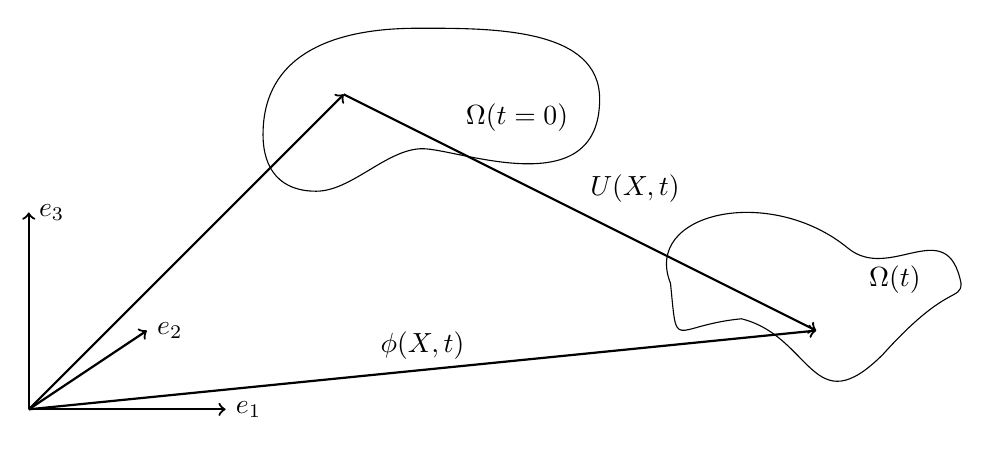
\begin{tikzpicture}
  %\draw[step=1.0,black,thin] (-3.,-1.) grid (3,4.);
  %\draw (-3,-1) -- (3,-1) -- (3,4) -- (-3,4) -- (-3,-1);
  \draw[thick,->] (-5,-2.5) -- (-2.5,-2.5) node [right] {$\vect{e}_1$};
  \draw[thick,->] (-5,-2.5) -- (-5,0.) node [right] {$\vect{e}_3$};
  \draw[thick,->] (-5,-2.5) -- (-3.5,-1.5) node [right] {$\vect{e}_2$};
  \begin{scope}[scale=0.45]
    \draw (-3,0.6) .. controls +(1,0) and +(-1,0) .. (0,1.8)  
    .. controls +(1,0) and +(0,-3) .. (5,3.2) 
    .. controls +(0,2) and +(2,0)  .. (0,5.2) 
    .. controls +(-1,0) and +(0,3) .. (-4.5,2.2) 
    .. controls +(0,-1) and +(-1,0).. (-3,0.6) ;
  \end{scope}
  \node at (1.2,1.2) {$\Omega(t=0)$};
  %% Deformed body +2.
  \begin{scope}[scale=0.9]
    \draw (0.+0.5+4.,0-1.5) ..controls (1.+0.5+4.,-0.25-1.5) and (1.+0.5+4.,-1.5-1.5) .. (2.+0.5+4.,-0.5-1.5) ..controls (2.9+0.5+4.,0.5-1.5) and (3.1+0.5+4.,0.25-1.5) .. (3.1+0.5+4.,0.5-1.5) ..controls (2.9+0.5+4.,1.5-1.5) and (2.1+0.5+4.,.5-1.5) .. (1.5+0.5+4.,1.-1.5) ..controls (0.4+0.5+4.,1.9-1.5) and (-1.4+0.5+4.,1.5-1.5) .. (-1.+0.5+4.,0.5-1.5)..controls (-0.4+0.+4.,-0.-2.) and (-1+0.5+4.,0.4-2.) .. (0+0.5+4.,0-1.5);
  \end{scope}
  \node at (6.,-0.85) {$\Omega(t)$};
  \draw[->,thick] (-5,-2.5) -- (-1.,1.5) node [midway,left] {$\X$};
  \draw[->,thick] (-5,-2.5) -- (5.,-1.5) node [midway,above] {$\vect{\phi}(\vect{X},t)$};
  \draw[->,thick] (-1.,1.5) -- (5.,-1.5) node [midway,above right] {$\vect{U}(\vect{X},t)$};
\end{tikzpicture}

%%% Local Variables:
%%% mode: latex
%%% TeX-master: "../../mainManuscript"
%%% End:
        \end{column}
        \begin{column}{0.5\textwidth}
          \begin{itemize}
          \item Reference mass density $\rho(\vect{X},t=0)=\rho_0(\vect{X})$
          \item Deformation gradient $\tens{F}(\vect{X},t)=\nablav_{\!0}\vect{\varphi}(\vect{X},t)$
          \item Cartesian coordinates system
          \end{itemize}
        \end{column}
      \end{columns}
    \end{block}
    \begin{block}{Balance equations \cite{Plohr}}
      \begin{equation*}
        \left.\begin{aligned}
            & \rho_0 \dot{\vect{v}} - \nablav_{\!0} \cdot \tens{\Pi} = \vect{0} \\
            & \dot{\tens{F}} - \nablav_{\!0} \cdot (\vect{v} \otimes \tens{I})= \tens{0}
          \end{aligned}\right\rbrace \Rightarrow \text{Conservative form: } \drond{\Ucb}{t} + \drond{\Fcb\cdot\vect{E}_\alpha}{X_\alpha} = \vect{0}
      \end{equation*}
      with $\Ucb = \matrice{\rho_0\vect{v} \\ \tens{F}} \: ; \: \Fcb\cdot\vect{E}_\alpha=\Fcb_\alpha=-\matrice{\tens{\Pi}\cdot\vect{E}_\alpha\\ \vect{v} \otimes\vect{E}_\alpha}$
    \end{block}
  \end{footnotesize}
  \footnoteCite{Plohr}
\end{frame}

\begin{frame}{Large deformations framework -- Constitutive equations}
  \begin{footnotesize}
    \begin{block}{Hyperelastic materials}
      %% Polyconvex, hyperbolicity ??
      From the thermodynamics: $\tens{\Pi}=\rho_0\drond{\psi}{\tens{F}}$ \\
      $\rho_0\psi$: Stored energy function, polyconvex $\Rightarrow$ hyperbolicity ensured \cite{Kluth}
    \end{block}
    \begin{block}{Quasi-linear form}
      Auxiliary vector $\Qcb$ \cite{Trangenstein91}: %$\Qcb=\matrice{\vect{v}\\\tens{\Pi}}$ 
      \begin{gather}
        % \dot{\tens{\Pi}} = \Hbb(\tens{F}) : \dot{\tens{F}} \Rightarrow \text{Quasi-linear form: } \drond{\Qcb}{t} + \Absf^\alpha \drond{\Qcb}{X_\alpha} = \vect{0}
        \drond{\Ucb}{t} + \drond{\Fcb\cdot\vect{E}_\alpha}{X_\alpha} = \vect{0} \quad \Leftrightarrow \quad \drond{\Ucb}{\alert{\Qcb}}\drond{\alert{\Qcb}}{t} + \drond{\Fcb\cdot\vect{E}_\alpha}{\alert{\Qcb}}\drond{\alert{\Qcb}}{X_\alpha}=\vect{0} \\
        \drond{\Qcb}{t} + \Absf^\alpha \drond{\Qcb}{X_\alpha} = \vect{0}
      \end{gather}
      where $\Qcb=\matrice{\vect{v}\\\tens{\Pi}} \: ; \: \Absf^\alpha = -\matrice{\tens{0}^2 & \frac{1}{\rho_0}\tens{I}\otimes\vect{E}_\alpha \\ \Hbb\cdot\vect{E}_\alpha & \tens{0}^4}$
    \end{block}
  \end{footnotesize}
  \footnoteCite{Kluth,Trangenstein91}
\end{frame}



\subsection{Discrete system}

\begin{frame}{Weak formulation}
  \begin{columns}
    \begin{column}{0.425\textwidth}
      \begin{block}{MPM space discretization}
        $N_p$ particles in $E$ elements
        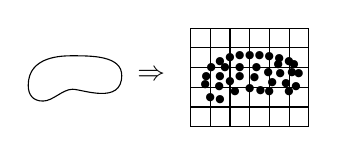
\begin{tikzpicture}[scale=0.25]
  % \draw[step=1.0,black,thin] (-3.,-1.) grid (3,4.);
  % \draw (-3,-1) -- (3,-1) -- (3,4) -- (-3,4) -- (-3,-1);
  \begin{scope}[scale=0.5]
    \draw (-3,0.6) .. controls +(1,0) and +(-1,0) .. (0,1.8)  
    .. controls +(1,0) and +(0,-3) .. (5,3.2) 
    .. controls +(0,2) and +(2,0)  .. (0,5.2) 
    .. controls +(-1,0) and +(0,3) .. (-4.5,2.2) 
    .. controls +(0,-1) and +(-1,0).. (-3,0.6) ;
    \begin{scope}  % pour limiter la portée du clip
      \clip (-3,0.6) .. controls +(1,0) and +(-1,0) .. (0,1.8) 
      .. controls +(1,0) and +(0,-3) .. (5,3.2)
      .. controls +(0,2) and +(2,0)  .. (0,5.2)
      .. controls +(-1,0) and +(0,3) .. (-4.5,2.2)
      .. controls +(0,-1) and +(-1,0).. (-3,0.6);
    \end{scope}
    %\node[below] at (0,1) {$\Omega$};
  \end{scope}
  \node at (4.,1.62) {$\Rightarrow$};
  \begin{scope}[shift={(9,0)}]
    \draw[step=1.0,black,thin] (-3.,-1.) grid (3,4.);
    % contour
    \node at (0,0.9) {\scriptsize$\bullet$}  ;
    \node at (2.5,1.65) {\scriptsize$\bullet$}  ; 
    \node at (0,2.6) {\scriptsize$\bullet$}  ;
    \node at (-2.25,1.1) {\scriptsize$\bullet$}  ; 
    \node at (-1.5,0.35) {\scriptsize$\bullet$}  ; 
    \node at (-2.,0.45) {\scriptsize$\bullet$} ;
    \node at (-2.2,1.5) {\scriptsize$\bullet$}  ; 
    \node at (-1.5,2.3) {\scriptsize$\bullet$} ; 
    \node at (2.35,1.) {\scriptsize$\bullet$}  ;
    \node at (2.25,2.15) {\scriptsize$\bullet$}  ;
    \node at (0.55,0.8) {\scriptsize$\bullet$}  ; 
    \node at (-0.5,2.6) {\scriptsize$\bullet$};
    \node at (0.5,2.59) {\scriptsize$\bullet$}  ;
    \node at (1.5,2.45) {\scriptsize$\bullet$}  ;
    \node at (1,0.75) {\scriptsize$\bullet$}; 
    \node at (2,0.75) {\scriptsize$\bullet$}  ;
    \node at (2,2.3) {\scriptsize$\bullet$}  ;
    \node at (1,2.55) {\scriptsize$\bullet$}  ;
    \node at (-1,2.5) {\scriptsize$\bullet$}  ; 
    \node at (-1.95,2.) {\scriptsize$\bullet$}  ;
    % interior
    \node at (-1.5,1.5) {\scriptsize$\bullet$}  ; 
    \node at (-1.25,2.) {\scriptsize$\bullet$}  ;
    \node at (-0.75,0.75) {\scriptsize$\bullet$}  ; 
    \node at (-1.55,1.){\scriptsize$\bullet$} ;
    \node at (-0.5,1.5) {\scriptsize$\bullet$}  ; 
    \node at (-0.5,2.) {\scriptsize$\bullet$}  ;
    \node at (0.25,1.45) {\scriptsize$\bullet$}  ;
    \node at (0.35,2.) {\scriptsize$\bullet$}  ;
    \node at (0.95,1.75) {\scriptsize$\bullet$}  ;
    \node at (1.15,1.2) {\scriptsize$\bullet$} ;
    \node at (1.45,2.15) {\scriptsize$\bullet$}  ; 
    \node at (1.55,1.65) {\scriptsize$\bullet$}  ;
    \node at (1.85,1.15) {\scriptsize$\bullet$}  ; 
    \node at (2.15,1.75) {\scriptsize$\bullet$}  ;
    \node at (-1.,1.25) {\scriptsize$\bullet$}  ;
    % \draw(3,0.5) -- (3.4,0.5) node [right]  {$\Omega_g$};
  \end{scope}
\end{tikzpicture}

%%% Local Variables:
%%% mode: latex
%%% TeX-master: "../presentation"
%%% End:

      \end{block}
    \end{column}
    \begin{column}{0.55\textwidth}
      \begin{block}{DG approximation \cite{DiPietro}}
        \vskip 14pt
        Broken polynomial space $\Vscr^k_h = \{\Vcb \in \Pscr^k(\Omega^e)\}$\\
        Approximate solution $\Ucb(\vect{X},t) \in \Vscr^k_h$ \\
        $\Vcb(\vect{X},t) = \sum_{i=1}^{N_{nodes}} S_i(\vect{X}) \Vcb^i(t)$
        \vskip 13pt
      \end{block}
    \end{column}
  \end{columns}
  \begin{block}{Element-wise weak form}
    \begin{equation*}
      \begin{aligned}
        & \text{Find $\Ucb\in \Vscr^1_h$ such that $\forall \:\Vcb,e,t \in \Vscr^1_h\times [1, E]\times \tau$:}\\
        & \int_{\Omega^e} \[\drond{\Ucb}{t} \Vcb - \Fcb_\alpha \drond{\Vcb}{X_\alpha}\]d\Omega + \int_{\partial \Omega^e} (\Fcb\cdot \vect{N}) d\Gamma = 0%\int_{\Omega^e} \Scb\Vcb d\Omega
      \end{aligned}
    \end{equation*}
  \end{block}
  \footnoteCite{DiPietro}
\end{frame}

\begin{frame}
  \begin{block}{Specific quantities}
    Approximation of the reference mass density \cite{Sulsky94}: $\rho_0(\vect{X})=\sum_{p=1}^{N_p}m_p \delta(\vect{X}^p-\vect{X})$ \\
    $\Rightarrow \: \Ucb = \rho_0 \bar{\Ucb} \:; \: \Fcb_\alpha = \rho_0 \bar{\Fcb}_\alpha$%\:; \: \Scb = \rho_0 \bar{\Scb}$
  \end{block}

  \begin{block}{Discrete weak form}
    \begin{equation*}
      \begin{aligned}
        & \text{Find $\Ucb\in \Vscr^1_h$ such that $\forall \:\Vcb,e,t \in \Vscr^1_h\times [1, E]\times \tau$:}\\
        & \sum_{p=1}^{N_p} m_p\[\ddroit{\bar{\Ucb}}{t} \Vcb - \bar{\Fcb}_\alpha \drond{\Vcb}{X_\alpha}\]_{\lvert_{\vect{X}=\vect{X}^p}} + \int_{\partial \Omega^e} (\Fcb\cdot \vect{N}) d\Gamma = \vect{0}
      \end{aligned}
    \end{equation*}
  \end{block}
  \footnoteCite{Sulsky94}
\end{frame}


\begin{frame}
  \begin{footnotesize}
    \begin{block}{Semi-discrete system}
      Introduction of polynomial approximation %$\Rightarrow  M_{ij} \ddroit{\bar{\Ucb}^j}{t}  - K_{ij}^\alpha \bar{\Fcb}^j_{\alpha} - \Scb^i + \hat{\Fcb}^i=  \vect{0} $
      \begin{equation*}
        M_{ij} \ddroit{\bar{\Ucb}^j}{t}  - K_{ij}^\alpha \bar{\Fcb}^j_{\alpha}  + \hat{\Fcb}^i=  \vect{0}
      \end{equation*}
      Diagonally lumped mass matrix $M^L_i=\sum_j M_{ij}$ \cite{Love}
    \end{block}
    \metroset{block=fill}
    \begin{block}{Explicit time discretization}
      \metroset{block=transparent}
      \begin{columns}
        \begin{column}{.4\textwidth}
          \begin{block}{\footnotesize Forward Euler}
            \vskip 7pt
            \begin{flalign*}
              M^L_i \frac{\bar{\Ucb}^{i,n+1} - \bar{\Ucb}^{i,n}}{\Delta t^n}=K_{ij}^\alpha \bar{\Fcb}^{j,n}_{\alpha}  - \hat{\Fcb}^{i,n}
            \end{flalign*}
            \vskip 14pt
          \end{block}
        \end{column}
        \begin{column}{.55\textwidth}
          \begin{block}{\footnotesize Second-order Runge-Kutta (RK2)}
            \vskip -5pt
            \begin{align*}
              & M^L_i \frac{\bar{\Ucb}^{i,n+1/2} - \bar{\Ucb}^{i,n}}{\Delta t^n}=\frac{1}{2}\(K_{ij}^\alpha \bar{\Fcb}^{j,n}_{\alpha}  - \hat{\Fcb}^{i,n}\) \\
              &M^L_i \frac{\bar{\Ucb}^{i,n+1} - \bar{\Ucb}^{i,n}}{\Delta t^n}=K_{ij}^\alpha \bar{\Fcb}^{j,n+1/2}_{\alpha}  - \hat{\Fcb}^{i,n+1/2}
            \end{align*}
          \end{block}
        \end{column}
      \end{columns}
    \end{block}
  \end{footnotesize}
  \footnoteCite{Love}
\end{frame}


\subsection{Interface fluxes}
\begin{frame}
  \begin{block}{Riemann problem}
    \begin{columns}
      \begin{column}{0.5\textwidth}
        \begin{footnotesize}
          \begin{align*}
          (\Rc\Pc): \quad &\drond{\Ucb}{t} + \drond{\Fcb_N}{\Ucb} \drond{\Ucb}{\xi }= \vect{0} \\ 
                          & \Ucb(\xi,0) = \left\lbrace 
                            \begin{aligned}
                              & \Ucb_L \: \text{if } \xi < 0 \\
                              & \Ucb_R \: \text{if } \xi > 0 
                            \end{aligned} \right.
          \end{align*}
        \end{footnotesize}
      \end{column}
      \begin{column}{0.3\textwidth}
        \begin{tikzpicture}[scale=0.5]
  \draw (10.,0.) -- (12.,6.) ; 
  \draw[fill=black] (9.85,0.1) circle (0.1) node [left] {$1$};	
  \draw[fill=black] (10.2,-0.0) circle (0.1) node [right] {$2$};	
  \draw[fill=black] (11.85,6.1) circle (0.1) node [left] {$4$};	
  \draw[fill=black] (12.2,6) circle (0.1) node [right] {$3$};	
  \draw[->,very thick] (11.,3.) -- (12,3 -1/3) node [right,below] {$X_N$}; 
  \node at (8,3.5) {$\vect{\Qc}_{L} = \frac{\vect{\Qc}_1 + \vect{\Qc}_4}{2}$}; \node at (14.5,3.5) {$\vect{\Qc}_{R} = \frac{\vect{\Qc}_2 + \vect{\Qc}_3}{2}$};
\end{tikzpicture}

      \end{column}
    \end{columns}
  \end{block}
  \begin{footnotesize}
    \begin{block}{Approximate Riemann solver \cite{Toro}}
      \begin{columns}
        \begin{column}{0.4\textwidth}
          \begin{itemize}
          \item Characteristic speeds $\lambda^i(\tens{F})$
          \item Simple waves
          \end{itemize}
        \end{column}  
        \begin{column}{0.55\textwidth}
          \begin{scriptsize}
  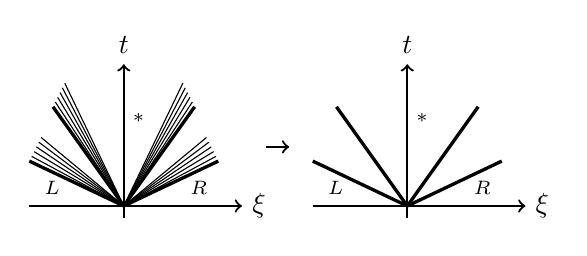
\begin{tikzpicture}[scale=0.3]
    \draw[->,thick] (-4,0) -- (5,0) node [right] {$\xi$};
    \draw[->,thick](0,-0.5) -- (0,6) node [above] {$t$};
    % Fastest left
    \draw[very thick](0,0) -- (-4,1.9) ;
    \draw(0,0) -- (-3.9,2.1) ;
    \draw(0,0) -- (-3.8,2.3) ;
    \draw(0,0) -- (-3.7,2.5) ;
    \draw(0,0) -- (-3.6,2.7) ;
    \draw(0,0) -- (-3.5,2.9) ;
    % Slowest left
    \draw[very thick](0,0) -- (-3.,4.2) ;
    \draw(0,0) -- (-2.9,4.4) ;
    \draw(0,0) -- (-2.8,4.6) ;
    \draw(0,0) -- (-2.7,4.8) ;
    \draw(0,0) -- (-2.6,5.0) ;
    \draw(0,0) -- (-2.5,5.2) ;
    % Fastest right
    \draw[very thick](0,0) -- (4,1.9) ;
    \draw(0,0) -- (3.9,2.1) ;
    \draw(0,0) -- (3.8,2.3) ;
    \draw(0,0) -- (3.7,2.5) ;
    \draw(0,0) -- (3.6,2.7) ;
    \draw(0,0) -- (3.5,2.9) ;
    % Slowest right
    \draw[very thick](0,0) -- (3.,4.2) ;
    \draw(0,0) -- (2.9,4.4) ;
    \draw(0,0) -- (2.8,4.6) ;
    \draw(0,0) -- (2.7,4.8) ;
    \draw(0,0) -- (2.6,5.0) ;
    \draw(0,0) -- (2.5,5.2) ;
    \node(a) at (-3,0.75) {$\Ucb_L$};
    \node(b) at (3.2,0.75) {$\Ucb_R$};
    \node(c) at (0.65,3.5) {$\Ucb^*$};
    \draw[->,thick](6.,2.5)--(7.,2.5) ;
    \begin{scope}[shift={(12.,0.)}]
      \draw[->,thick] (-4,0) -- (5,0) node [right] {$\xi$};
      \draw[->,thick](0,-0.5) -- (0,6) node [above] {$t$};
      % Fastest left
      \draw[very thick](0,0) -- (-4,1.9) ;
      % Slowest left
      \draw[very thick](0,0) -- (-3.,4.2) ;
      % Fastest right
      \draw[very thick](0,0) -- (4,1.9) ;
      % Slowest right
      \draw[very thick](0,0) -- (3.,4.2) ;
      \node(a) at (-3,0.75) {$\Ucb_L$};
      \node(b) at (3.2,0.75) {$\Ucb_R$};
      \node(c) at (0.65,3.5) {$\Ucb^*$};
    \end{scope}
  \end{tikzpicture}
\end{scriptsize}

%%% Local Variables:
%%% mode: latex
%%% TeX-master: "../../presentation"
%%% End:
        \end{column}
      \end{columns}
    \end{block}
    Computation of $\Ucb^* \Rightarrow$ corresponding (Godunov) flux: $\vect{\Fc}_N(\Ucb^*)$\\
    \alert{Integration of constitutive equations}
    
  \end{footnotesize}
   \footnoteCite{Toro}
 \end{frame}

\begin{frame}%{\normalsize Boundary conditions}
  \begin{block}{\footnotesize Boundary Conditions: ghost nodes}
    \begin{columns}
      \begin{column}{0.3\textwidth}
        \begin{scriptsize}
  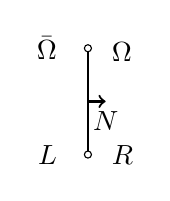
\begin{tikzpicture}[scale=0.45]
    \draw[thick] (0.0,0.0) -- (0,-3) ;
    \draw[->,thick] (0,-1.5) -- (0.5,-1.5) node [below] {$\vect{N}$};
    %\draw[->] (0,-1.5) -- (1,-1.5) node [below] {$\xi$};
    \node[left] at (-0.6,-3) {$L$};
    \node[right] at (.4,-3) {$R$};
    \node[left] at (-0.6,0) {$\bar{\Omega}$};
    \node[right] at (.4,-0.1) {$\Omega$};
    \draw [fill=white] (0,0) circle (0.1);
    \draw [fill=white] (0,-3) circle (0.1);
  \end{tikzpicture}	
\end{scriptsize}

%%% Local Variables:
%%% mode: latex
%%% TeX-master: "../../presentation"
%%% End:
      \end{column}
      \begin{column}{0.6\textwidth}
        \begin{scriptsize}
          \begin{itemize}
          \item[] Enforce $\Ucb_L$ such that $\Ucb^*=\Ucb^{imp}$
          \item[] Problem: apply strain rather than stress 
          \end{itemize}
        \end{scriptsize}
      \end{column}	
    \end{columns}
  \end{block}
  \begin{scriptsize}
  $\Rightarrow $ Quasi-linear form with suitable $\Qcb$ (\textit{i.e. containing stress})\\
  \alert{Also avoid the integration of constitutive equations at element interfaces !}
  \end{scriptsize}
  \begin{block}{\footnotesize Transverse corrections: Adaptation of the Corner Transport Upwind method \cite{Colella_CTU}}
    \centering
    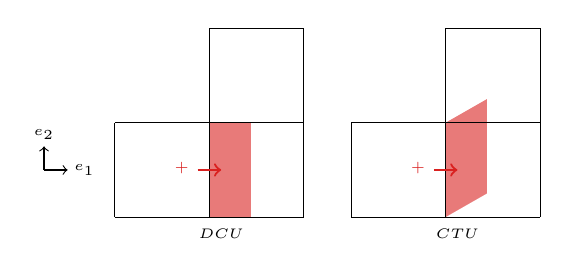
\begin{tikzpicture}[scale=0.6]
  \fill[Red!60] (0,0) rectangle (.875,-2);
  \draw (-2,0) -- (2,0.);\draw (0.,2) -- (0,-2.);\draw (0,2) -- (2,2);
  \draw (-2.,-2.) -- (2.,-2.);\draw (2,2.) -- (2,-2.);\draw (-2,-2) -- (-2,0);
  \begin{tiny}
    \draw[->,thick,Red] (-.25,-1.) node [left] {$\Ac^+$} -- (.25,-1.) ;
    \draw[->] (-3.5,-1.) -- (-3,-1.) node[right] {$\vect{e}_1$};
    \draw[->] (-3.5,-1.) -- (-3.5,-0.5) node[above] {$\vect{e}_2$};
    \node at (0.25,-2.35) {$DCU$};
  \end{tiny}
  \begin{scope}[shift={(5.,0.)}]
    \fill[Red!60] (0,0) rectangle (.875,-2);
    \fill[Red!60] (0,0) -- (.875,0) -- (.875,.5) -- (0.,0.); %% Red triangle
    \fill[white] (0,0-2) -- (.875,0-2) -- (.875,.5-2) -- (0.,0.-2); %% White triangle
    \draw (-2,0) -- (2,0.);\draw (0.,2) -- (0,-2.);\draw (0,2) -- (2,2);
    \draw (-2.,-2.) -- (2.,-2.);\draw (2,2.) -- (2,-2.);\draw (-2,-2) -- (-2,0);
    \begin{tiny}
      \draw[->,thick,Red] (-.25,-1.) node [left] {$\Ac^+$} -- (.25,-1.) ;
      \node at (0.25,-2.35) {$CTU$};
    \end{tiny}    
  \end{scope}
\end{tikzpicture}

%%% Local Variables:
%%% mode: latex
%%% TeX-master: "../../presentation"
%%% End:

  \end{block}
  \footnoteCite{Colella_CTU}
\end{frame}

\subsection{Solution scheme}
%\begin{frame}{Procedure between $t^n$ and $t^n + \Delta t^n=t^{n+1}$}
  \begin{footnotesize}
    \begin{overprint}
      %% Computation of matrices
      \onslide<1>
      \begin{equation*}
        \text{Discrete system: }\alert{M^L_{i}} \frac{\bar{\Ucb}^{i,n+1} - \bar{\Ucb}^{i,n}}{\Delta t^n}  - \alert{K_{ij}^\alpha} \bar{\Fcb}^{j,n}_{\alpha}  + \hat{\Fcb}^{i,n}=  \vect{0}
      \end{equation*}
      \begin{columns}
        \begin{column}{0.4\textwidth}
          \begin{itemize}
          \item[(1)] Computation of matrices $M_i^L$ and $K_{ij}^\alpha$
          \end{itemize}
        \end{column}
        \vrule{}
        \begin{column}{0.6\textwidth}
          \begin{block}{Computation of matrices $M_i^L$ and $K_{ij}^\alpha$}
            \begin{columns}
              \begin{column}{0.3\textwidth}
                \vskip 0.9pt
                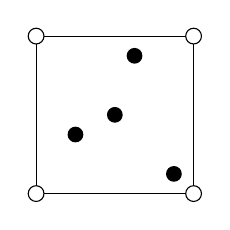
\begin{tikzpicture}
                  \draw (0,0) rectangle (2,2);
                  \fill[white] (0,0) circle (0.1); \fill[white] (0,2) circle (0.1); \fill[white] (2,0) circle (0.1); \fill[white] (2,2) circle (0.1);
                  \draw (0,0) circle (0.1); \draw (0,2) circle (0.1); \draw (2,0) circle (0.1); \draw (2,2) circle (0.1);
                  \fill[black] (0.5,0.75) circle (0.1); \fill[black] (1.25,1.75) circle (0.1); \fill[black] (1.75,0.25) circle (0.1); \fill[black] (1,1) circle (0.1);
                \end{tikzpicture}
              \end{column}
              \begin{column}{0.6\textwidth}
                States of particles known at time $t^n$:
                \begin{equation*}
                  \left\lbrace\begin{aligned}
                      & \vect{v}^{p,n},\tens{F}^{p,n},\tens{\Pi}^{p,n} \: \rightarrow \:\Ucb^{p,n},\Qcb^{p,n}\\
                      & \vect{X}^{p,n} \: \rightarrow \:M_i^{L,n},K_{ij}^{\alpha,n}
                    \end{aligned}\right.
                \end{equation*}
                
              \end{column}
            \end{columns}
          \end{block}
        \end{column}
      \end{columns}

      %% Particles -> Nodes
      \onslide<2>
      \begin{equation*}
        \text{Discrete system: }M^L_{i} \frac{\bar{\Ucb}^{i,n+1} - \alert{\bar{\Ucb}^{i,n}}}{\Delta t^n}  - K_{ij}^\alpha \bar{\Fcb}^{j,n}_{\alpha}  + \hat{\Fcb}^{i,n}=  \vect{0}
      \end{equation*}
      \begin{columns}
        \begin{column}{0.4\textwidth}
          \begin{itemize}
          \item[(1)] Computation of matrices $M_i^L$ and $K_{ij}^\alpha$
          \item[(2)] Projection particles $\rightarrow$ nodes
          \end{itemize}
        \end{column}
        \vrule{}
        \begin{column}{0.6\textwidth}
          \begin{block}{Projection particles $\rightarrow$ nodes}
            \begin{columns}
              \begin{column}{0.3\textwidth}
                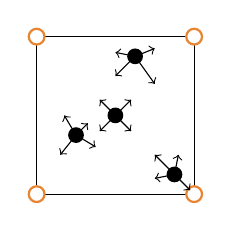
\begin{tikzpicture}
                  \draw (0,0) rectangle (2,2);
                  \fill[white] (0,0) circle (0.1); \fill[white] (0,2) circle (0.1); \fill[white] (2,0) circle (0.1); \fill[white] (2,2) circle (0.1);
                  \draw[Orange,thick] (0,0) circle (0.1); \draw[Orange,thick] (0,2) circle (0.1); \draw[Orange,thick] (2,0) circle (0.1); \draw[Orange,thick] (2,2) circle (0.1);
                  \fill[black] (0.5,0.75) circle (0.1); \fill[black] (1.25,1.75) circle (0.1); \fill[black] (1.75,0.25) circle (0.1); \fill[black] (1,1) circle (0.1);
                  %% North arrows
                  \draw[->,black] (1.25,1.75) -- (1.5,1.85);\draw[->,black] (1.25,1.75) -- (1.,1.8);\draw[->,black] (1.25,1.75) -- (1.,1.5);\draw[->,black] (1.25,1.75) -- (1.5,1.4);
                  %% West arrows
                  \draw[->,black] (0.5,0.75) -- (0.3,0.5);\draw[->,black] (0.5,0.75) -- (0.35,1.);\draw[->,black] (0.5,0.75) -- (0.75,.6);\draw[->,black] (0.5,0.75) -- (.65,0.9);
                  %% Center arrows
                  \draw[->,black] (1,1) -- (1.2,1.2);\draw[->,black] (1,1) -- (1.2,0.8);\draw[->,black] (1,1) -- (0.8,1.2);\draw[->,black] (1,1) -- (0.8,0.8);
                  %% South arrows
                  \draw[->,black] (1.75,0.25) -- (1.95,.05);\draw[->,black] (1.75,0.25) -- (1.8,.5);\draw[->,black] (1.75,0.25) -- (1.5,.5);\draw[->,black] (1.75,0.25) -- (1.5,0.2);
                \end{tikzpicture}
              \end{column}
              \begin{column}{0.6\textwidth}
                \begin{equation*}
                  \begin{aligned}
                    & M^{L,n}_i \alert{\bar{\Ucb}^{i,n}} = \sum_{p=1}^{N_p} m_p \bar{\Ucb}^{p,n}\\
                    & M^{L,n}_i \alert{\Qcb^{i,n}} = \sum_{p=1}^{N_p} m_p \Qcb^{p,n}
                  \end{aligned}
                \end{equation*}
              \end{column}
            \end{columns}
          \end{block}
        \end{column}
      \end{columns}
      
      %% Computation of numerical fluxes (volume + intercell)
      \onslide<3>
      \begin{equation*}
        \text{Discrete system: }M^L_{i} \frac{\bar{\Ucb}^{i,n+1} - \bar{\Ucb}^{i,n}}{\Delta t^n}  - K_{ij}^\alpha \alert{\bar{\Fcb}^{j,n}_{\alpha}}  + \alert{\hat{\Fcb}^{i,n}}=  \vect{0}
      \end{equation*}
      \begin{columns}
        \begin{column}{0.4\textwidth}
          \begin{itemize}
          \item[(1)] Computation of matrices $M_i^L$ and $K_{ij}^\alpha$
          \item[(2)] Projection particles $\rightarrow$ nodes
          \item[(3)] Computation of fluxes
          \end{itemize}
        \end{column}
        \vrule{}
        \begin{column}{0.6\textwidth}
          \begin{block}{Computation of fluxes}
            \begin{columns}
              \begin{column}{0.4\textwidth}
                \begin{block}{\footnotesize Volume fluxes}
                  $\bar{\Ucb}^{i,n},\Qcb^{i,n} \rightarrow \bar{\Fcb}^{i,n}_\alpha$
                \end{block}
              \end{column}
              \begin{column}{0.55\textwidth}
                \begin{block}{\footnotesize Intercell fluxes}
                  Approximate Riemann solver $\rightarrow \hat{\Fcb}^i$
                \end{block}
              \end{column}
            \end{columns}
          \end{block}
        \end{column}
      \end{columns}
      
      %% Time integration + Interpolation
      \onslide<4>
      \begin{equation*}
        \text{Discrete system: }M^L_{i} \frac{\alert{\bar{\Ucb}^{i,n+1}} - \bar{\Ucb}^{i,n}}{\Delta t^n}  - K_{ij}^\alpha \bar{\Fcb}^{j,n}_{\alpha}  + \hat{\Fcb}^{i,n}=  \vect{0}
      \end{equation*}
      \begin{columns}
        \begin{column}{0.4\textwidth}
          \begin{itemize}
          \item[(1)] Computation of matrices $M_i^L$ and $K_{ij}^\alpha$
          \item[(2)] Projection particles $\rightarrow$ nodes
          \item[(3)] Computation of fluxes
          \item[(4)] Explicit time integration; Interpolation
          \end{itemize}
        \end{column}
        \vrule{}
        \begin{column}{0.6\textwidth}
          \begin{block}{Explicit time integration; Interpolation}
            
            \begin{columns}
              \begin{column}{0.4\textwidth}
                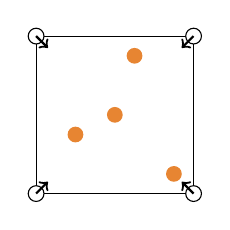
\begin{tikzpicture}
                  \draw (0,0) rectangle (2,2);
                  \fill[white] (0,0) circle (0.1); \fill[white] (0,2) circle (0.1); \fill[white] (2,0) circle (0.1); \fill[white] (2,2) circle (0.1);
                  \draw (0,0) circle (0.1); \draw (0,2) circle (0.1); \draw (2,0) circle (0.1); \draw (2,2) circle (0.1);
                  \draw[->,thick] (0,0) -- (0.15,0.15);
                  \draw[->,thick] (2,0) -- (1.85,0.15);
                  \draw[->,thick] (2,2) -- (1.85,1.85);
                  \draw[->,thick] (0,2) -- (.15,1.85);
                  
                  \fill[Orange] (0.5,0.75) circle (0.1); \fill[Orange] (1.25,1.75) circle (0.1); \fill[Orange] (1.75,0.25) circle (0.1); \fill[Orange] (1,1) circle (0.1);
                  
                  % \fill[black!50] (0.5,0.75) circle (0.1); \fill[black!50] (1.25,1.75) circle (0.1); \fill[black!50] (1.75,0.25) circle (0.1); \fill[black!50] (1,1) circle (0.1);
                  % \fill[black] (0.75,1.25) circle (0.1); \fill[black] (1.75,2.25) circle (0.1); \fill[black] (2.1,0.75) circle (0.1); \fill[black] (1.5,1.5) circle (0.1);
                  % \path[->,thick,black] (0.5,0.75) edge[bend left] (0.73,1.22);
                  % \path[->,thick,black] (1.25,1.75) edge[bend right] (1.75,2.21);
                  % \path[->,thick,black](1.75,0.25) edge[bend left] (2.,0.75);
                  % \path[->,thick,black](1,1) edge[bend right] (1.5,1.4);
                \end{tikzpicture}
              \end{column}
              \begin{column}{0.55\textwidth}
                \begin{equation*}
                  \alert{\bar{\Ucb}^{p,n+1}}=\sum_{i=1}^{N_{nodes}} S_{i}(\vect{X}^{p}) \bar{\Ucb}^{i,n+1}
                \end{equation*}
              \end{column}
            \end{columns}
          \end{block}
        \end{column}
      \end{columns}
           
      %% Kinematic and constitutive updates
      \onslide<5>
      \begin{columns}
        \begin{column}{0.4\textwidth}
          \begin{itemize}
          \item[(1)] Computation of matrices $M_i^L$ and $K_{ij}^\alpha$
          \item[(2)] Projection particles $\rightarrow$ nodes
          \item[(3)] Computation of fluxes
          \item[(4)] Explicit time integration; Interpolation
          \item[(5)] Kinematics and constitutive updates
          \end{itemize}
        \end{column}
        \vrule{}
        \begin{column}{0.6\textwidth}
          \begin{block}{Kinematics and constitutive updates}
            \begin{columns}
              \begin{column}{0.4\textwidth}
                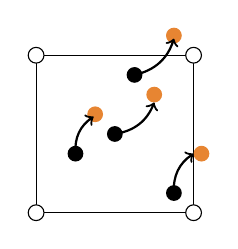
\begin{tikzpicture}
                  \draw (0,0) rectangle (2,2);
                  \fill[white] (0,0) circle (0.1); \fill[white] (0,2) circle (0.1); \fill[white] (2,0) circle (0.1); \fill[white] (2,2) circle (0.1);
                  \draw (0,0) circle (0.1); \draw (0,2) circle (0.1); \draw (2,0) circle (0.1); \draw (2,2) circle (0.1);
                  \fill[black] (0.5,0.75) circle (0.1); \fill[black] (1.25,1.75) circle (0.1); \fill[black] (1.75,0.25) circle (0.1); \fill[black] (1,1) circle (0.1);
                  \fill[Orange] (0.75,1.25) circle (0.1); \fill[Orange] (1.75,2.25) circle (0.1); \fill[Orange] (2.1,0.75) circle (0.1); \fill[Orange] (1.5,1.5) circle (0.1);
                  \path[->,thick,black] (0.5,0.75) edge[bend left] (0.73,1.22);
                  \path[->,thick,black] (1.25,1.75) edge[bend right] (1.75,2.21);
                  \path[->,thick,black](1.75,0.25) edge[bend left] (2.,0.75);
                  \path[->,thick,black](1,1) edge[bend right] (1.5,1.4);
                \end{tikzpicture}
              \end{column}
              \begin{column}{0.55\textwidth}
                \begin{flalign*}
                  \begin{aligned}
                    & \alert{\tens{\Pi}^{p,n+1}}=g(\tens{F}^{p,n+1})\\
                    & \alert{\vect{\varphi}^{p,n+1}}= \vect{\varphi}^{p,n} +\Delta t^n \vect{v}^{p,n+1}
                  \end{aligned}
                \end{flalign*}
              \end{column}
            \end{columns}
          \end{block}
        \end{column}
      \end{columns}
      
      
      %% Rebuild the grid if needed
      \onslide<6>
      \begin{columns}
        \begin{column}{0.4\textwidth}
          \begin{itemize}
          \item[(1)] Computation of matrices $M_i^L$ and $K_{ij}^\alpha$
          \item[(2)] Projection particles $\rightarrow$ nodes
          \item[(3)] Computation of fluxes
          \item[(4)] Explicit time integration; Interpolation
          \item[(5)] Kinematics and constitutive updates
          \item[(6)] Reconstruction of the grid (if needed) 
          \end{itemize}
        \end{column}
        \vrule{}
        \begin{column}{0.6\textwidth}
          \begin{block}{Reconstruction of the grid (if needed)}
            \begin{columns}
              \begin{column}{0.4\textwidth}
                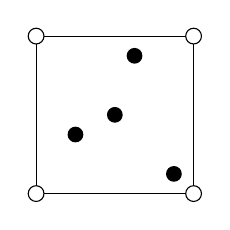
\begin{tikzpicture}
                  \draw (0,0) rectangle (2,2);
                  \fill[white] (0,0) circle (0.1); \fill[white] (0,2) circle (0.1); \fill[white] (2,0) circle (0.1); \fill[white] (2,2) circle (0.1);
                  \draw (0,0) circle (0.1); \draw (0,2) circle (0.1); \draw (2,0) circle (0.1); \draw (2,2) circle (0.1);
                  \fill[black] (0.5,0.75) circle (0.1); \fill[black] (1.25,1.75) circle (0.1); \fill[black] (1.75,0.25) circle (0.1); \fill[black] (1,1) circle (0.1);
                \end{tikzpicture}
              \end{column}
              \begin{column}{0.55\textwidth}
                \centering
                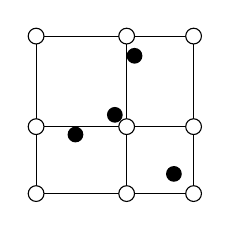
\begin{tikzpicture}
                  \draw (0,0) rectangle (2.,2.);
                  \draw (1.15,0.85) rectangle (2.,0);
                  \draw (1.15,0.85) rectangle (2.,2);
                  \draw (1.15,0.85) rectangle (0.,2);
                  %% Old nodes
                  \fill[white] (0,0) circle (0.1);
                  \fill[white] (0,2) circle (0.1);
                  \fill[white] (2,0) circle (0.1);
                  \fill[white] (2,2) circle (0.1);
                  \draw (0,0) circle (0.1);
                  \draw (0,2) circle (0.1);
                  \draw (2,0) circle (0.1);
                  \draw (2,2) circle (0.1);

                  %% Added nodes
                  \fill[white] (1.15,0.85) circle (0.1);
                  \fill[white] (0,0.85) circle (0.1);
                  \fill[white] (2,0.85) circle (0.1);
                  \fill[white] (1.15,0) circle (0.1);
                  \fill[white] (1.15,2) circle (0.1);
                  \draw (1.15,0.85) circle (0.1);
                  \draw (0,0.85) circle (0.1);
                  \draw (2,0.85) circle (0.1);
                  \draw (1.15,0) circle (0.1);
                  \draw (1.15,2) circle (0.1);

                  %% Particles
                  \fill[black] (0.5,0.75) circle (0.1); \fill[black] (1.25,1.75) circle (0.1); \fill[black] (1.75,0.25) circle (0.1); \fill[black] (1,1) circle (0.1);
                \end{tikzpicture}
              \end{column}
            \end{columns}
          \end{block}
        \end{column}
      \end{columns}
    \end{overprint}
  \end{footnotesize}
\end{frame}

\begin{frame}{Procedure between $t^n$ and $t^n + \Delta t^n=t^{n+1}$}
  \begin{footnotesize}
    %% Computation of matrices
    \begin{equation*}
      \text{Discrete system: }\alert{M^L_{i}} \frac{\bar{\Ucb}^{i,n+1} - \bar{\Ucb}^{i,n}}{\Delta t^n}  - \alert{K_{ij}^\alpha} \bar{\Fcb}^{j,n}_{\alpha}  + \hat{\Fcb}^{i,n}=  \vect{0}
    \end{equation*}
    \begin{columns}
      \begin{column}{0.4\textwidth}
        \begin{itemize}
        \item[(1)] Computation of matrices $M_i^L$ and $K_{ij}^\alpha$
        \end{itemize}
      \end{column}
      \vrule{}
      \begin{column}{0.6\textwidth}
        \begin{block}{Computation of matrices $M_i^L$ and $K_{ij}^\alpha$}
          \begin{columns}
            \begin{column}{0.3\textwidth}
              \vskip 0.9pt
              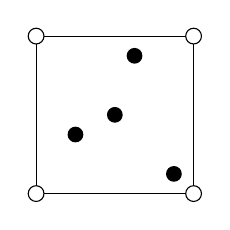
\begin{tikzpicture}
                \draw (0,0) rectangle (2,2);
                \fill[white] (0,0) circle (0.1); \fill[white] (0,2) circle (0.1); \fill[white] (2,0) circle (0.1); \fill[white] (2,2) circle (0.1);
                \draw (0,0) circle (0.1); \draw (0,2) circle (0.1); \draw (2,0) circle (0.1); \draw (2,2) circle (0.1);
                \fill[black] (0.5,0.75) circle (0.1); \fill[black] (1.25,1.75) circle (0.1); \fill[black] (1.75,0.25) circle (0.1); \fill[black] (1,1) circle (0.1);
              \end{tikzpicture}
            \end{column}
            \begin{column}{0.6\textwidth}
              States of particles known at time $t^n$:
              \begin{equation*}
                \left\lbrace\begin{aligned}
                    & \vect{v}^{p,n},\tens{F}^{p,n},\tens{\Pi}^{p,n} \: \rightarrow \:\Ucb^{p,n},\Qcb^{p,n}\\
                    & \vect{X}^{p,n} \: \rightarrow \:M_i^{L,n},K_{ij}^{\alpha,n}
                  \end{aligned}\right.
              \end{equation*}
              
            \end{column}
          \end{columns}
        \end{block}
      \end{column}
    \end{columns}
  \end{footnotesize}
\end{frame}

\begin{frame}{Procedure between $t^n$ and $t^n + \Delta t^n=t^{n+1}$}
  \begin{footnotesize}
    %% Particles -> Nodes
    \begin{equation*}
      \text{Discrete system: }M^L_{i} \frac{\bar{\Ucb}^{i,n+1} - \alert{\bar{\Ucb}^{i,n}}}{\Delta t^n}  - K_{ij}^\alpha \bar{\Fcb}^{j,n}_{\alpha}  + \hat{\Fcb}^{i,n}=  \vect{0}
    \end{equation*}
    \begin{columns}
      \begin{column}{0.4\textwidth}
        \begin{itemize}
        \item[(1)] Computation of matrices $M_i^L$ and $K_{ij}^\alpha$
        \item[(2)] Projection particles $\rightarrow$ nodes
        \end{itemize}
      \end{column}
      \vrule{}
      \begin{column}{0.6\textwidth}
        \begin{block}{Projection particles $\rightarrow$ nodes}
          \begin{columns}
            \begin{column}{0.3\textwidth}
              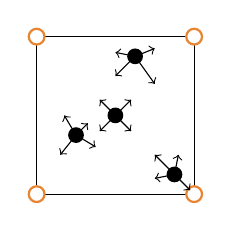
\begin{tikzpicture}
                \draw (0,0) rectangle (2,2);
                \fill[white] (0,0) circle (0.1); \fill[white] (0,2) circle (0.1); \fill[white] (2,0) circle (0.1); \fill[white] (2,2) circle (0.1);
                \draw[Orange,thick] (0,0) circle (0.1); \draw[Orange,thick] (0,2) circle (0.1); \draw[Orange,thick] (2,0) circle (0.1); \draw[Orange,thick] (2,2) circle (0.1);
                \fill[black] (0.5,0.75) circle (0.1); \fill[black] (1.25,1.75) circle (0.1); \fill[black] (1.75,0.25) circle (0.1); \fill[black] (1,1) circle (0.1);
                %% North arrows
                \draw[->,black] (1.25,1.75) -- (1.5,1.85);\draw[->,black] (1.25,1.75) -- (1.,1.8);\draw[->,black] (1.25,1.75) -- (1.,1.5);\draw[->,black] (1.25,1.75) -- (1.5,1.4);
                %% West arrows
                \draw[->,black] (0.5,0.75) -- (0.3,0.5);\draw[->,black] (0.5,0.75) -- (0.35,1.);\draw[->,black] (0.5,0.75) -- (0.75,.6);\draw[->,black] (0.5,0.75) -- (.65,0.9);
                %% Center arrows
                \draw[->,black] (1,1) -- (1.2,1.2);\draw[->,black] (1,1) -- (1.2,0.8);\draw[->,black] (1,1) -- (0.8,1.2);\draw[->,black] (1,1) -- (0.8,0.8);
                %% South arrows
                \draw[->,black] (1.75,0.25) -- (1.95,.05);\draw[->,black] (1.75,0.25) -- (1.8,.5);\draw[->,black] (1.75,0.25) -- (1.5,.5);\draw[->,black] (1.75,0.25) -- (1.5,0.2);
              \end{tikzpicture}
            \end{column}
            \begin{column}{0.6\textwidth}
              \begin{equation*}
                \begin{aligned}
                  & M^{L,n}_i \alert{\bar{\Ucb}^{i,n}} = \sum_{p=1}^{N_p} m_p \bar{\Ucb}^{p,n}\\
                  & M^{L,n}_i \alert{\Qcb^{i,n}} = \sum_{p=1}^{N_p} m_p \Qcb^{p,n}
                \end{aligned}
              \end{equation*}
            \end{column}
          \end{columns}
        \end{block}
      \end{column}
    \end{columns}
  \end{footnotesize}
\end{frame}


\begin{frame}{Procedure between $t^n$ and $t^n + \Delta t^n=t^{n+1}$}
  \begin{footnotesize}
    %% Computation of numerical fluxes (volume + intercell)
    \begin{equation*}
      \text{Discrete system: }M^L_{i} \frac{\bar{\Ucb}^{i,n+1} - \bar{\Ucb}^{i,n}}{\Delta t^n}  - K_{ij}^\alpha \alert{\bar{\Fcb}^{j,n}_{\alpha}}  + \alert{\hat{\Fcb}^{i,n}}=  \vect{0}
    \end{equation*}
    \begin{columns}
      \begin{column}{0.4\textwidth}
        \begin{itemize}
        \item[(1)] Computation of matrices $M_i^L$ and $K_{ij}^\alpha$
        \item[(2)] Projection particles $\rightarrow$ nodes
        \item[(3)] Computation of fluxes
        \end{itemize}
      \end{column}
      \vrule{}
      \begin{column}{0.6\textwidth}
        \begin{block}{Computation of fluxes}
          \begin{columns}
            \begin{column}{0.4\textwidth}
              \begin{block}{\footnotesize Volume fluxes}
                $\bar{\Ucb}^{i,n},\Qcb^{i,n} \rightarrow \bar{\Fcb}^{i,n}_\alpha$
              \end{block}
            \end{column}
            \begin{column}{0.55\textwidth}
              \begin{block}{\footnotesize Intercell fluxes}
                Approximate Riemann solver $\rightarrow \hat{\Fcb}^i$
              \end{block}
            \end{column}
          \end{columns}
        \end{block}
      \end{column}
    \end{columns}
  \end{footnotesize}
\end{frame}

\begin{frame}{Procedure between $t^n$ and $t^n + \Delta t^n=t^{n+1}$}
  \begin{footnotesize}
    %% Time integration + Interpolation
    \begin{equation*}
      \text{Discrete system: }M^L_{i} \frac{\alert{\bar{\Ucb}^{i,n+1}} - \bar{\Ucb}^{i,n}}{\Delta t^n}  - K_{ij}^\alpha \bar{\Fcb}^{j,n}_{\alpha}  + \hat{\Fcb}^{i,n}=  \vect{0}
    \end{equation*}
    \begin{columns}
      \begin{column}{0.4\textwidth}
        \begin{itemize}
        \item[(1)] Computation of matrices $M_i^L$ and $K_{ij}^\alpha$
        \item[(2)] Projection particles $\rightarrow$ nodes
        \item[(3)] Computation of fluxes
        \item[(4)] Explicit time integration; Interpolation
        \end{itemize}
      \end{column}
      \vrule{}
      \begin{column}{0.6\textwidth}
        \begin{block}{Explicit time integration; Interpolation}
          
          \begin{columns}
            \begin{column}{0.4\textwidth}
              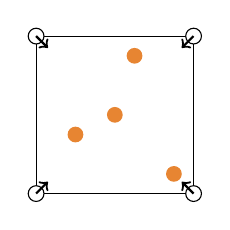
\begin{tikzpicture}
                \draw (0,0) rectangle (2,2);
                \fill[white] (0,0) circle (0.1); \fill[white] (0,2) circle (0.1); \fill[white] (2,0) circle (0.1); \fill[white] (2,2) circle (0.1);
                \draw (0,0) circle (0.1); \draw (0,2) circle (0.1); \draw (2,0) circle (0.1); \draw (2,2) circle (0.1);
                \draw[->,thick] (0,0) -- (0.15,0.15);
                \draw[->,thick] (2,0) -- (1.85,0.15);
                \draw[->,thick] (2,2) -- (1.85,1.85);
                \draw[->,thick] (0,2) -- (.15,1.85);
                
                \fill[Orange] (0.5,0.75) circle (0.1); \fill[Orange] (1.25,1.75) circle (0.1); \fill[Orange] (1.75,0.25) circle (0.1); \fill[Orange] (1,1) circle (0.1);
              \end{tikzpicture}
            \end{column}
            \begin{column}{0.55\textwidth}
              \begin{equation*}
                \alert{\bar{\Ucb}^{p,n+1}}=\sum_{i=1}^{N_{nodes}} S_{i}(\vect{X}^{p}) \bar{\Ucb}^{i,n+1}
              \end{equation*}
            \end{column}
          \end{columns}
        \end{block}
      \end{column}
    \end{columns}
  \end{footnotesize}
\end{frame}

\begin{frame}{Procedure between $t^n$ and $t^n + \Delta t^n=t^{n+1}$}
  \begin{footnotesize}
    %% Kinematic and constitutive updates
    \begin{columns}
      \begin{column}{0.4\textwidth}
        \begin{itemize}
        \item[(1)] Computation of matrices $M_i^L$ and $K_{ij}^\alpha$
        \item[(2)] Projection particles $\rightarrow$ nodes
        \item[(3)] Computation of fluxes
        \item[(4)] Explicit time integration; Interpolation
        \item[(5)] Kinematics and constitutive updates
        \end{itemize}
      \end{column}
      \vrule{}
      \begin{column}{0.6\textwidth}
        \begin{block}{Kinematics and constitutive updates}
          \begin{columns}
            \begin{column}{0.4\textwidth}
              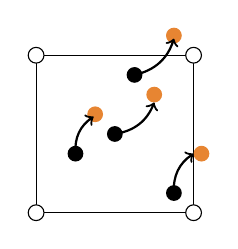
\begin{tikzpicture}
                \draw (0,0) rectangle (2,2);
                \fill[white] (0,0) circle (0.1); \fill[white] (0,2) circle (0.1); \fill[white] (2,0) circle (0.1); \fill[white] (2,2) circle (0.1);
                \draw (0,0) circle (0.1); \draw (0,2) circle (0.1); \draw (2,0) circle (0.1); \draw (2,2) circle (0.1);
                \fill[black] (0.5,0.75) circle (0.1); \fill[black] (1.25,1.75) circle (0.1); \fill[black] (1.75,0.25) circle (0.1); \fill[black] (1,1) circle (0.1);
                \fill[Orange] (0.75,1.25) circle (0.1); \fill[Orange] (1.75,2.25) circle (0.1); \fill[Orange] (2.1,0.75) circle (0.1); \fill[Orange] (1.5,1.5) circle (0.1);
                \path[->,thick,black] (0.5,0.75) edge[bend left] (0.73,1.22);
                \path[->,thick,black] (1.25,1.75) edge[bend right] (1.75,2.21);
                \path[->,thick,black](1.75,0.25) edge[bend left] (2.,0.75);
                \path[->,thick,black](1,1) edge[bend right] (1.5,1.4);
              \end{tikzpicture}
            \end{column}
            \begin{column}{0.55\textwidth}
              \begin{flalign*}
                \begin{aligned}
                  & \alert{\tens{\Pi}^{p,n+1}}=g(\tens{F}^{p,n+1})\\
                  & \alert{\vect{\varphi}^{p,n+1}}= \vect{\varphi}^{p,n} +\Delta t^n \vect{v}^{p,n+1}
                \end{aligned}
              \end{flalign*}
            \end{column}
          \end{columns}
        \end{block}
      \end{column}
    \end{columns}
  \end{footnotesize}
\end{frame}
      
\begin{frame}{Procedure between $t^n$ and $t^n + \Delta t^n=t^{n+1}$}
  \begin{footnotesize}
    %% Rebuild the grid if needed
    \begin{columns}
      \begin{column}{0.4\textwidth}
        \begin{itemize}
        \item[(1)] Computation of matrices $M_i^L$ and $K_{ij}^\alpha$
        \item[(2)] Projection particles $\rightarrow$ nodes
        \item[(3)] Computation of fluxes
        \item[(4)] Explicit time integration; Interpolation
        \item[(5)] Kinematics and constitutive updates
        \item[(6)] Reconstruction of the grid (if needed) 
        \end{itemize}
      \end{column}
      \vrule{}
      \begin{column}{0.6\textwidth}
        \begin{block}{Reconstruction of the grid (if needed)}
          \begin{columns}
            \begin{column}{0.4\textwidth}
              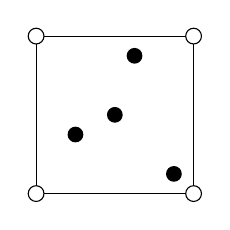
\begin{tikzpicture}
                \draw (0,0) rectangle (2,2);
                \fill[white] (0,0) circle (0.1); \fill[white] (0,2) circle (0.1); \fill[white] (2,0) circle (0.1); \fill[white] (2,2) circle (0.1);
                \draw (0,0) circle (0.1); \draw (0,2) circle (0.1); \draw (2,0) circle (0.1); \draw (2,2) circle (0.1);
                \fill[black] (0.5,0.75) circle (0.1); \fill[black] (1.25,1.75) circle (0.1); \fill[black] (1.75,0.25) circle (0.1); \fill[black] (1,1) circle (0.1);
              \end{tikzpicture}
            \end{column}
            \begin{column}{0.55\textwidth}
              \centering
              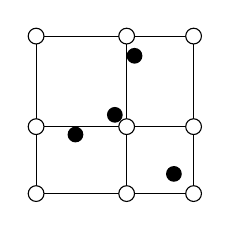
\begin{tikzpicture}
                \draw (0,0) rectangle (2.,2.);
                \draw (1.15,0.85) rectangle (2.,0);
                \draw (1.15,0.85) rectangle (2.,2);
                \draw (1.15,0.85) rectangle (0.,2);
                %% Old nodes
                \fill[white] (0,0) circle (0.1);
                \fill[white] (0,2) circle (0.1);
                \fill[white] (2,0) circle (0.1);
                \fill[white] (2,2) circle (0.1);
                \draw (0,0) circle (0.1);
                \draw (0,2) circle (0.1);
                \draw (2,0) circle (0.1);
                \draw (2,2) circle (0.1);
                
                %% Added nodes
                \fill[white] (1.15,0.85) circle (0.1);
                \fill[white] (0,0.85) circle (0.1);
                \fill[white] (2,0.85) circle (0.1);
                \fill[white] (1.15,0) circle (0.1);
                \fill[white] (1.15,2) circle (0.1);
                \draw (1.15,0.85) circle (0.1);
                \draw (0,0.85) circle (0.1);
                \draw (2,0.85) circle (0.1);
                \draw (1.15,0) circle (0.1);
                \draw (1.15,2) circle (0.1);
                
                %% Particles
                \fill[black] (0.5,0.75) circle (0.1); \fill[black] (1.25,1.75) circle (0.1); \fill[black] (1.75,0.25) circle (0.1); \fill[black] (1,1) circle (0.1);
              \end{tikzpicture}
            \end{column}
          \end{columns}
        \end{block}
      \end{column}
    \end{columns}
  \end{footnotesize}
\end{frame}
%%% Local Variables:
%%% mode: latex
%%% TeX-master: "../presentation"
%%% End:


%%% Local Variables:
%%% mode: latex
%%% TeX-master: "../presentation"
%%% End:



\section{Numerical analysis}
\subsection{Stability analysis}
\begin{frame}{Linear advection equation of an arbitrary quantity $q$}%{One-dimensional problems}
  \begin{block}{Scheme equation (finite difference sense)}
    \begin{footnotesize}
      \begin{equation*}
        \bar{q}^{p,n+1}=\sum_{k=1}^{N_p}H_{pk}(\vect{X}^p,\vect{X}^k,CFL)\bar{q}^{k,n}
      \end{equation*}
    \end{footnotesize}
  \end{block}
  \begin{block}{von-Neumann linear stability analysis}
    \begin{footnotesize}
      The numerical scheme is stable if:
      \begin{equation*}
        \sum_{k=1}^{N_p}\abs{H_{pk}} \leq 1 \quad \forall p
      \end{equation*}
      \alert{$\Rightarrow$ find the maximal $CFL$ number ensuring the stability}
    \end{footnotesize}
  \end{block}\pause
  \metroset{block=fill}
  \begin{footnotesize}
    \begin{block}{Particular case: one particle per cell}
      The first-order FVM is recovered $\rightarrow$ CFL improved compared to MPM 
    \end{block}
    %Comment on CTU + other discretizations
  \end{footnotesize}
  %% Reformuler cette slide sans equation ou alors ecrire le grand principe de minimisation de la fonctionnelle dont l'argument est le CFL pour laisser de la place aux commentaires sur les discrétisations
\end{frame}

\subsection{Convergence analysis}
\begin{frame}
  \begin{block}{\footnotesize Elastic one-dimensional bar -- small strains}
    \begin{columns}
      \begin{column}{0.45\textwidth}
        \centering
        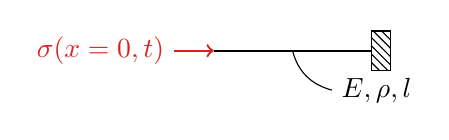
\begin{tikzpicture}
          \draw[thick] (0,0) -- (2,0);
          \draw[pattern=north west lines] (2,-0.25) rectangle (2.25,0.25);
          \draw[->,Red,thick] (-.5,0) node[left] {$\sigma(x=0,t)$} -- (0,0);
          \path (1.,0) edge[bend right] (1.5,-0.5) ;
          \node[right] at (1.5,-0.5) {$E,\rho,l$};
        \end{tikzpicture}
      \end{column}
      \begin{column}{0.45\textwidth}
        $\sigma(x=0,t) = \sigma^d \sin\(\frac{0.4\pi}{l} \sqrt{\frac{E}{\rho}}\:t\)$
      \end{column}
    \end{columns}
  \end{block}
  \begin{overprint}
    \onslide<1>
    %% Graph pour 2ppc regularly spaced
    \begin{block}{\footnotesize $L^2$ relative error -- two particles per cell}
      \begin{columns}
        \begin{column}{0.49\textwidth}
          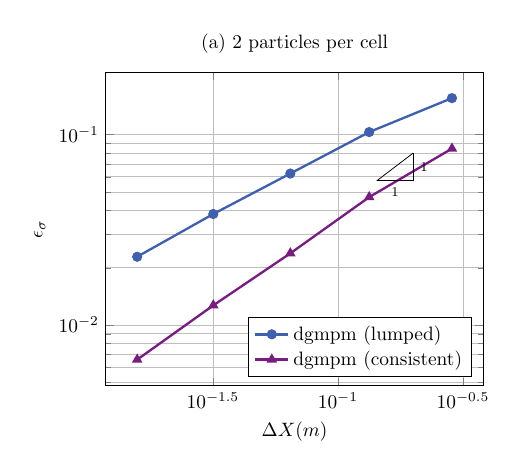
\begin{tikzpicture}[scale=0.7]
\begin{loglogaxis}[xlabel=$\Delta X (m)$,ylabel=$\epsilon_\sigma$,ymajorgrids=true,xmajorgrids=true,legend pos=south east,title={(a) 2 particles per cell}]
\addplot[Blue,very thick,mark=*] coordinates {(0.285714285714,0.155344401413) (0.133333333333,0.103056278416) (0.0645161290323,0.0624467155513) (0.031746031746,0.0383032357895) (0.0157480314961,0.0228383166886) };
\addlegendentry{dgmpm (lumped)}
\addplot[Purple,very thick,mark=triangle*] coordinates {(0.285714285714,0.0844046229439) (0.133333333333,0.0469432859143) (0.0645161290323,0.0238077178296) (0.031746031746,0.0126928564059) (0.0157480314961,0.0065867196308) };
\addlegendentry{dgmpm (consistent)}
\draw (axis cs:0.2,0.08) -- (axis cs:0.2/1.4,0.08/1.4);
\draw (axis cs:0.2,0.08) -- (axis cs:0.2,0.08/1.4) node [midway,right] {\scriptsize 1};
\draw (axis cs:0.2,0.08/1.4) -- (axis cs:0.2/1.4,0.08/1.4) node [midway,below] {\scriptsize 1};
\end{loglogaxis}
\end{tikzpicture}

        \end{column}
        \begin{column}{0.49\textwidth}
          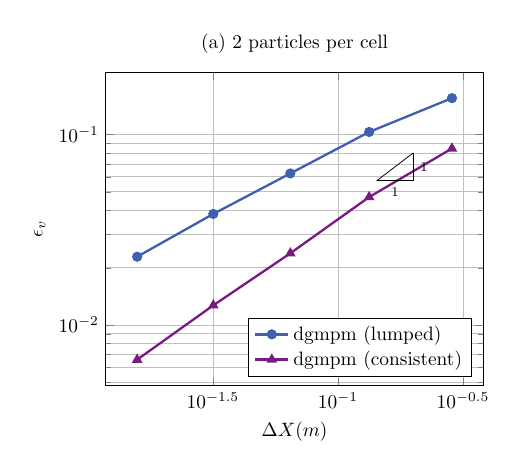
\begin{tikzpicture}[scale=0.7]
\begin{loglogaxis}[xlabel=$\Delta X (m)$,ylabel=$\epsilon_v$,ymajorgrids=true,xmajorgrids=true,legend pos=south east,title={(a) 2 particles per cell}]
\addplot[Blue,very thick,mark=*] coordinates {(0.285714285714,0.155081880585) (0.133333333333,0.103056265942) (0.0645161290323,0.0624467155504) (0.031746031746,0.0383032357895) (0.0157480314961,0.0228383166886) };
\addlegendentry{dgmpm (lumped)}
\addplot[Purple,very thick,mark=triangle*] coordinates {(0.285714285714,0.0844044636359) (0.133333333333,0.0469432859143) (0.0645161290323,0.0238077178296) (0.031746031746,0.0126928564059) (0.0157480314961,0.0065867196308) };
\addlegendentry{dgmpm (consistent)}
\draw (axis cs:0.2,0.08) -- (axis cs:0.2/1.4,0.08/1.4);
\draw (axis cs:0.2,0.08) -- (axis cs:0.2,0.08/1.4) node [midway,right] {\scriptsize 1};
\draw (axis cs:0.2,0.08/1.4) -- (axis cs:0.2/1.4,0.08/1.4) node [midway,below] {\scriptsize 1};
\end{loglogaxis}
\end{tikzpicture}

        \end{column}
      \end{columns}
    \end{block}

    \onslide<2>
    %% Tableau pour les autres
    \begin{block}{\footnotesize $L^2$ relative error -- other space discretizations}
      \centering
      \vskip 10pt
      \begin{footnotesize}
          \begin{tabular}{c|cc|cc|cc|cc}
    \hline
    PPC & \multicolumn{2}{c}{DGMPM--Euler}  \vline & \multicolumn{2}{c}{DGMPM--RK2}\vline  & \multicolumn{2}{c}{MPM} \vline & \multicolumn{2}{c}{MPM--PIC}  \\ [6pt]
    & $\sigma$ & $v$  & $\sigma$ & $v$  & $\sigma$ & $v$ & $\sigma$ & $v$\\ 
    \hline
    \hline
    2 & 0.63 & 0.63 & 0.80 &0.80 & 0.88 & 1.46&0.94& 0.85\\
    6 & 0.66 & 0.66 & 0.91 &0.91 &  0.91&1.62&1.07&0.92\\
    10 & 0.67 & 0.67 & 0.93 &0.93 &0.92&1.62&1.10&0.92\\
    20 & 0.68 & 0.67 & 0.95 &0.95 &0.92&1.61&1.12&0.93\\
    \hline
  \end{tabular}

%%% Local Variables:
%%% mode: latex
%%% TeX-master: "../../mainManuscript"
%%% End:

      \end{footnotesize}
      
    \end{block}
  \end{overprint}
  
\end{frame}

%%% Local Variables:
%%% mode: latex
%%% TeX-master: "../presentation"
%%% End:



\section{Numerical simulations}
\begin{frame}[plain]{Outline}
  \tableofcontents[currentsection,hideothersubsections]
\end{frame}


\subsection{Linearized geometrical framework}
\begin{frame}{\href{section4/animation/elasticity_stress/video.mp4}{Plane strain elasticity}}
  \begin{overprint}
    \onslide<1>
    \vspace{-1.cm}
    \begin{columns}
      \begin{column}{0.42\linewidth}
        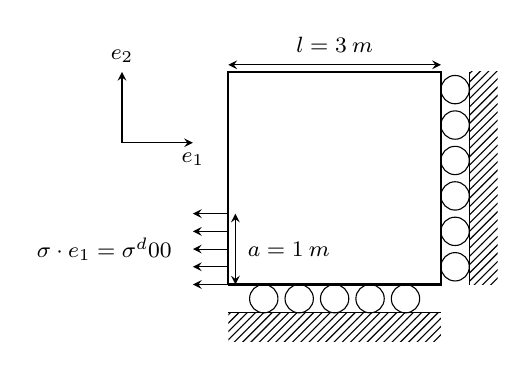
\begin{tikzpicture}[scale=0.9]
  \draw[thick] (0,0) --(3,0)--(3,3)--(0,3)--(0,0);
  \foreach \x in {0.5,1.,...,2.5} 
  \draw(\x,-0.2)circle(0.2);
  \foreach \x in {0.25,0.75,...,2.75} 
  \draw(3.2,\x)circle(0.2);
  \draw(0,-0.4)--(3.,-0.4);
  \draw(3.4,0)--(3.4,3);
  \fill [pattern=north east lines](0.0,-0.8)rectangle+(3,0.4);
  \fill [pattern=north east lines](3.4,0.)rectangle+(0.4,3);
  \draw[>=stealth,<->](0,3.1)--node[above=1pt]{\footnotesize $l=3 \: m$}(3,3.1);
  \draw[>=stealth,<->](0.1,0)--node[right=1pt]{\footnotesize $a=1 \: m$}(0.1,1);
  \foreach \x in {0.,0.25,...,1} 
  \draw[>=stealth,<-] (-0.5,\x)--(0.,\x);
  \node(a)at(-1.75,0.5){\footnotesize $\tens{\sigma}\cdot\vect{e}_1=\matrice{\sigma^d\\0 \\0}$}; 
  \draw[>=stealth,->](-1.5,2)--(-0.5,2)node(a)[anchor=north]{\footnotesize $\vect{e}_1$};
  \draw[>=stealth,->](-1.5,2)--(-1.5,3)node(a)[anchor=south]{\footnotesize $\vect{e}_2$};
\end{tikzpicture}


%%% Local Variables:
%%% mode: latex
%%% TeX-master: "../../mainManuscript"
%%% End:

      \end{column}

      \begin{column}{0.6\linewidth}
        \vspace{1.5cm}
        \centering
        \phantom{\begin{tikzpicture}
  \begin{groupplot}[group style={group size=2 by 1,
ylabels at=edge left, yticklabels at=edge left,horizontal sep=3.ex,
xticklabels at=edge bottom,xlabels at=edge bottom},
ymajorgrids=true,xmajorgrids=true,ylabel=$\sigma_{12} \: (Pa)$,
axis on top,scale only axis,width=0.4\linewidth, every x tick scale label/.style={at={(xticklabel* cs:1.05,0.75cm)},anchor=near yticklabel},ymin=-0.5e6,ymax=.5e9]
\nextgroupplot[ylabel=$\sigma_{11} (Pa)$,xlabel=$x (m)$]
\addplot[Red,very thick,no markers] table[x=Points:0,y=S11] {chapter4/csvFiles/2delast_fem_115.csv};
\addplot[Blue,very thick,mark=+,only marks,mark size=3pt] table[x=Points:0,y=stress_11] {chapter4/csvFiles/2delast_ctu1ppc_115.csv};
\addplot[Purple,very thick,mark=square*,only marks] table[x=Points:0,y=stress_11] {chapter4/csvFiles/2delast_ctu4ppc_115.csv};
\addplot[Orange,very thick,mark=x,only marks,mark size=3pt] table[x=Points:0,y=mpm_S11] {chapter4/csvFiles/2delast_mpm_115.csv};

\nextgroupplot[legend style={at={($(0.12,-0.35)+(0.9cm,1cm)$)},legend columns=2},xlabel=$x (m)$]
\addplot[Red,very thick,no markers] table[x=Points:0,y=S11] {chapter4/csvFiles/2delast_fem_338.csv};
\addplot[Blue,very thick,mark=+,only marks,mark size=3pt] table[x=Points:0,y=stress_11] {chapter4/csvFiles/2delast_ctu1ppc_338.csv};
\addplot[Purple,very thick,mark=square*,only marks] table[x=Points:0,y=stress_11] {chapter4/csvFiles/2delast_ctu4ppc_338.csv};
\addplot[Orange,very thick,mark=x,only marks,mark size=3pt] table[x=Points:0,y=mpm_S11] {chapter4/csvFiles/2delast_mpm_338.csv};
\addlegendentry{fem}
\addlegendentry{ctu 1ppc}
\addlegendentry{ctu 4ppc}
\addlegendentry{mpm}
   
  \end{groupplot}
\end{tikzpicture}


%%% Local Variables:
%%% mode: latex
%%% TeX-master: "../../mainManuscript"
%%% End:




































%%% Local Variables:
%%% mode: latex
%%% TeX-master: "../../mainManuscript"
%%% End:
}
      \end{column}
      
    \end{columns}
    \onslide<2>
    \vspace{-1.cm}
    \begin{columns}
      \begin{column}{0.42\linewidth}
        \movie[height=.7\paperheight,width=1.\linewidth,showcontrols,loop,poster,autostart]{%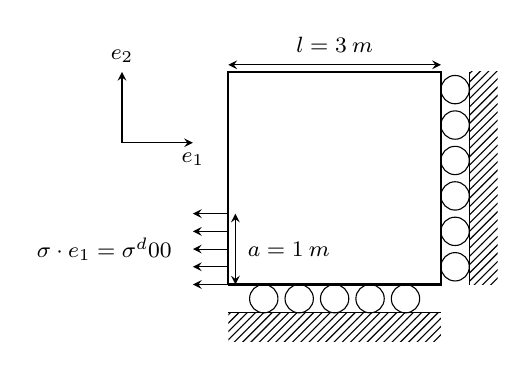
\begin{tikzpicture}[scale=0.9]
  \draw[thick] (0,0) --(3,0)--(3,3)--(0,3)--(0,0);
  \foreach \x in {0.5,1.,...,2.5} 
  \draw(\x,-0.2)circle(0.2);
  \foreach \x in {0.25,0.75,...,2.75} 
  \draw(3.2,\x)circle(0.2);
  \draw(0,-0.4)--(3.,-0.4);
  \draw(3.4,0)--(3.4,3);
  \fill [pattern=north east lines](0.0,-0.8)rectangle+(3,0.4);
  \fill [pattern=north east lines](3.4,0.)rectangle+(0.4,3);
  \draw[>=stealth,<->](0,3.1)--node[above=1pt]{\footnotesize $l=3 \: m$}(3,3.1);
  \draw[>=stealth,<->](0.1,0)--node[right=1pt]{\footnotesize $a=1 \: m$}(0.1,1);
  \foreach \x in {0.,0.25,...,1} 
  \draw[>=stealth,<-] (-0.5,\x)--(0.,\x);
  \node(a)at(-1.75,0.5){\footnotesize $\tens{\sigma}\cdot\vect{e}_1=\matrice{\sigma^d\\0 \\0}$}; 
  \draw[>=stealth,->](-1.5,2)--(-0.5,2)node(a)[anchor=north]{\footnotesize $\vect{e}_1$};
  \draw[>=stealth,->](-1.5,2)--(-1.5,3)node(a)[anchor=south]{\footnotesize $\vect{e}_2$};
\end{tikzpicture}


%%% Local Variables:
%%% mode: latex
%%% TeX-master: "../../mainManuscript"
%%% End:

        }{section4/animation/elasticity_stress/video.mp4}
      \end{column}

      \begin{column}{0.6\linewidth}
        \vspace{1.5cm}
        \centering
        \begin{tikzpicture}
  \begin{groupplot}[group style={group size=2 by 1,
ylabels at=edge left, yticklabels at=edge left,horizontal sep=3.ex,
xticklabels at=edge bottom,xlabels at=edge bottom},
ymajorgrids=true,xmajorgrids=true,ylabel=$\sigma_{12} \: (Pa)$,
axis on top,scale only axis,width=0.4\linewidth, every x tick scale label/.style={at={(xticklabel* cs:1.05,0.75cm)},anchor=near yticklabel},ymin=-0.5e6,ymax=.5e9]
\nextgroupplot[ylabel=$\sigma_{11} (Pa)$,xlabel=$x (m)$]
\addplot[Red,very thick,no markers] table[x=Points:0,y=S11] {chapter4/csvFiles/2delast_fem_115.csv};
\addplot[Blue,very thick,mark=+,only marks,mark size=3pt] table[x=Points:0,y=stress_11] {chapter4/csvFiles/2delast_ctu1ppc_115.csv};
\addplot[Purple,very thick,mark=square*,only marks] table[x=Points:0,y=stress_11] {chapter4/csvFiles/2delast_ctu4ppc_115.csv};
\addplot[Orange,very thick,mark=x,only marks,mark size=3pt] table[x=Points:0,y=mpm_S11] {chapter4/csvFiles/2delast_mpm_115.csv};

\nextgroupplot[legend style={at={($(0.12,-0.35)+(0.9cm,1cm)$)},legend columns=2},xlabel=$x (m)$]
\addplot[Red,very thick,no markers] table[x=Points:0,y=S11] {chapter4/csvFiles/2delast_fem_338.csv};
\addplot[Blue,very thick,mark=+,only marks,mark size=3pt] table[x=Points:0,y=stress_11] {chapter4/csvFiles/2delast_ctu1ppc_338.csv};
\addplot[Purple,very thick,mark=square*,only marks] table[x=Points:0,y=stress_11] {chapter4/csvFiles/2delast_ctu4ppc_338.csv};
\addplot[Orange,very thick,mark=x,only marks,mark size=3pt] table[x=Points:0,y=mpm_S11] {chapter4/csvFiles/2delast_mpm_338.csv};
\addlegendentry{fem}
\addlegendentry{ctu 1ppc}
\addlegendentry{ctu 4ppc}
\addlegendentry{mpm}
   
  \end{groupplot}
\end{tikzpicture}


%%% Local Variables:
%%% mode: latex
%%% TeX-master: "../../mainManuscript"
%%% End:




































%%% Local Variables:
%%% mode: latex
%%% TeX-master: "../../mainManuscript"
%%% End:

      \end{column}
    \end{columns}
  \end{overprint}
\end{frame}


\begin{frame}{Plane strain elastoplasticity}
  \begin{overprint}
    \onslide<1>
    \vspace{0.25cm}
    \centering
    \movie[height=.7\paperheight,width=.75\linewidth,showcontrols,loop,poster,autostart]{
    }{section4/animation/elastoplasticity/video.ogv}
    \onslide<2>
    \centering
    \begin{tikzpicture}
  \begin{groupplot}[group style={group size=2 by 1,
ylabels at=edge left, yticklabels at=edge left,horizontal sep=3.ex,
xticklabels at=edge bottom,xlabels at=edge bottom},
ymajorgrids=true,xmajorgrids=true,ymin=-0.1e-3,ymax=6.75e-3,
axis on top,scale only axis,width=0.4\linewidth, every x tick scale label/.style={at={(xticklabel* cs:1.05,0.75cm)},anchor=near yticklabel}]
\nextgroupplot[ylabel=$\eps^p_{11}$,xlabel=$x (m)$]
\addplot[Red,very thick,no markers] table[x=Points:0,y=EP11] {appendix/csvFiles/2dEP_fem_115.csv};
\addplot[Blue,very thick,mark=+,only marks,mark size=3pt] table[x=Points:0,y=epsp_11] {appendix/csvFiles/2dEP_ctu1ppc_115.csv};
\addplot[Purple,very thick,mark=square*,only marks] table[x=Points:0,y=epsp_11] {appendix/csvFiles/2dEP_ctu4ppc_115.csv};
\addplot[Orange,very thick,mark=x,only marks,mark size=3pt] table[x=Points:0,y= mpm_epsp11] {appendix/csvFiles/2dEP_mpm_115.csv};

\nextgroupplot[legend style={at={($(0.12,-0.35)+(0.9cm,1cm)$)},legend columns=2},xlabel=$x (m)$]
\addplot[Red,very thick,no markers] table[x=Points:0,y=EP11] {appendix/csvFiles/2dEP_fem_338.csv};
\addplot[Blue,very thick,mark=+,only marks,mark size=3pt] table[x=Points:0,y=epsp_11] {appendix/csvFiles/2dEP_ctu1ppc_338.csv};
\addplot[Purple,very thick,mark=square*,only marks] table[x=Points:0,y=epsp_11] {appendix/csvFiles/2dEP_ctu4ppc_338.csv};
\addplot[Orange,very thick,mark=x,only marks,mark size=3pt] table[x=Points:0,y= mpm_epsp11] {appendix/csvFiles/2dEP_mpm_338.csv};
\addlegendentry{fem}
\addlegendentry{ctu 1ppc}
\addlegendentry{ctu 4ppc}
\addlegendentry{mpm}
   
  \end{groupplot}
\end{tikzpicture}


%%% Local Variables:
%%% mode: latex
%%% TeX-master: "../../mainManuscript"
%%% End:




































%%% Local Variables:
%%% mode: latex
%%% TeX-master: "../../mainManuscript"
%%% End:

  \end{overprint}

\end{frame}
%%% Local Variables:
%%% mode: latex
%%% TeX-master: "../aRenaud"
%%% End:
\subsection{Large strains framework}
\begin{frame}{Hyperelastic plane wave -- Neo-Hookean material}
  \begin{columns}
    \begin{column}{.5\linewidth}
      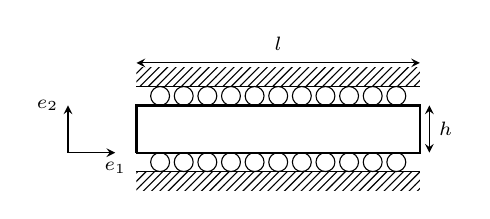
\begin{tikzpicture}[scale=0.6]
  % \draw[thick] (0,0) --(4,0)--(4,3)--(0,3)--(0,0);
  \draw[thick] (0,0) --(6,0)--(6,1)--(0,1)--(0,0);
  \foreach \x in {0.5,1.,...,5.5} 
  \draw(\x,-0.2)circle(0.2);
  \foreach \x in {0.5,1.,...,5.5} 
  \draw(\x,1.2)circle(0.2);
  \draw(0,-0.4)--(6.,-0.4);
  \draw(0,1.4)--(6.,1.4);
  \fill [pattern=north east lines](0.0,-0.8)rectangle+(6.,0.4);
  \fill [pattern=north east lines](0.,1.4)rectangle+(6.,0.4);
  \draw[>=stealth,<->](6.2,0)--node[right]{\scriptsize $h$}(6.2,1.);
  \draw[>=stealth,<->](0,1.9)--node[above=1pt]{\scriptsize$l$}(6,1.9);
  \draw[>=stealth,->](-3.2+1.75,0.)--(-2.2+1.75,0.)node(a)[anchor=north]{\scriptsize$\vect{e}_1$};
  \draw[>=stealth,->](-3.2+1.75,0.)--(-3.2+1.75,1)node(a)[anchor=east]{\scriptsize$\vect{e}_2$};
\end{tikzpicture}

%%% Local Variables:
%%% mode: latex
%%% TeX-master: "../../presentation"
%%% End:

      a préciser car vitesse initiale (à voir d'ailleurs car ça n'apporte pas grand chose...)
    \end{column}

    \begin{column}{.5\linewidth}
      \begin{tikzpicture}[scale=.8]
\begin{axis}[xlabel=$time (s)$,ylabel=$\frac{e}{e_{max}}$,ymajorgrids=true,xmajorgrids=true,legend pos=outer north east,title={},legend style={at={($(0.1,-0.35)+(0.5cm,1cm)$)},legend columns=2}]%legend pos=outer north east
\addplot[Red,very thick,mark=none,dashed,mark size=3pt] coordinates {(9.000573014794848e-06,1.0) (1.796381527756706e-05,0.9914533911626189) (2.6909286505214812e-05,0.9880756808914547) (3.585756699770927e-05,0.9854163150120561) (4.4822911312038465e-05,0.9789097295366027) (5.378423847837861e-05,0.9708660526421296) (6.273631604137162e-05,0.9656702364262686) (7.169197372887131e-05,0.9625409739506655) (8.066025051487872e-05,0.9574679354059819) (8.961671522275958e-05,0.9500647102454508) (9.857118385750588e-05,0.9437541147042068) (0.00010753083860163041,0.9398798249683428) (0.00011649057391700033,0.9356832648318265) (0.0001254456574397425,0.9291492959903835) (0.00013440464853789163,0.9222530895675854) (0.0001433667710713556,0.9174592561135397) (0.00015232285930250012,0.9135982466881382) (0.00016128049723290437,0.9080047243813228) (0.00017024437615889375,0.9010493561227031) (0.00017920147124044156,0.8953825087396217) (0.00018815854511947014,0.8913497349914383) (0.00019712199080299233,0.8865572214476816) (0.00020607998559766153,0.8800037607395182) (0.0002150368836279206,0.8736769151351442) (0.0002239987476753767,0.8691054692043627) (0.00023295751227616783,0.8648169199264896) (0.00024191442874660712,0.8589184707817774) (0.00025087522253969616,0.8522957120637725) };
\addplot[Orange,very thick,mark=none,densely dotted,mark size=3pt] coordinates {(1.8001146029589695e-05,1.0) (3.59337432830172e-05,0.987287010657628) (5.38434339576714e-05,0.9814549372480271) (7.177081672658308e-05,0.970637903879259) (8.968366215918615e-05,0.9554754935028931) (0.00010757624410062916,0.9454593249947213) (0.0001254888371660142,0.9382623428226724) (0.00014341501849920492,0.9259931945416342) (0.00016132703431225403,0.9120343329658626) (0.00017924741148391378,0.9029541004990023) (0.00019716238450120902,0.8947404029938869) (0.00021508320559939724,0.8818562426281039) (0.0002330026139290141,0.8689169578863969) (0.0002509126129702663,0.8603520482744869) };
\addplot[Purple,thick,mark=x,solid,mark size=3pt] coordinates {(7.314899467950566e-06,1.0) (1.4598146985673229e-05,0.9901528409608024) (2.186753874650882e-05,0.9809991185505665) (2.9130901458336235e-05,0.9721874325775748) (3.63916412745582e-05,0.9635884129780377) (4.365124162858778e-05,0.9551376250276616) (5.0910347345400474e-05,0.9467976667376566) (5.8169238149383194e-05,0.9385446028223614) (6.542803550311455e-05,0.9303620393969964) (7.268679212790383e-05,0.9222381699438393) (7.994553091400178e-05,0.9141641574908818) (8.72042617922543e-05,0.9061331831412421) (9.446298907826645e-05,0.8981398539433616) (0.00010172171466011121,0.890179817127578) (0.00010898043935922209,0.8822494990710554) (0.00011623916354340497,0.874345922941322) (0.00012349788737204238,0.8664665778426528) (0.00013075661094321585,0.858609322671656) (0.00013801533428144574,0.850772314137439) (0.00014527405742351267,0.8429539517751796) (0.00015253278038167682,0.8351528354294445) (0.00015979150316819838,0.8273677318145014) (0.00016705022578307734,0.8195975479492331) (0.0001743089482508341,0.8118413097554148) (0.00018156767057146868,0.8040981447385332) (0.0001888263927572412,0.7963672677259795) (0.00019608511482041192,0.7886479691085402) (0.00020334383676098083,0.7809396050484623) (0.0002106025585789479,0.7732415892416323) (0.00021786128028657335,0.7655533859586525) (0.00022512000188385718,0.7578745041586655) (0.00023237872338305955,0.7502044924212865) (0.0002396374447841805,0.7425429346279839) (0.00024689616608722,0.7348894462080099) (0.00025415488730443824,0.7272436708773569) };
\addplot[Green,very thick,mark=+,solid,mark size=3pt] coordinates {(5.8804885337294695e-06,1.0) (1.174826095073322e-05,0.9871640924586731) (1.7607631385637616e-05,0.9762308082517568) (2.3460937455554108e-05,0.9662965796826042) (2.9309741742850362e-05,0.9569353639389021) (3.515517745412317e-05,0.9479551306920194) (4.0998087388800795e-05,0.9392550356546122) (4.683910268494923e-05,0.930772911643581) (5.267869681390552e-05,0.9224666140508109) (5.851722504021463e-05,0.9143059680447483) (6.435495392470625e-05,0.9062685194043427) (7.019208344645524e-05,0.8983370369661849) (7.602876357621121e-05,0.8904979605583739) (8.186510678872026e-05,0.88274039349438) (8.77011974127584e-05,0.8750554248472826) (9.353709865908055e-05,0.8674356582122611) (9.93728579048248e-05,0.8598748748510392) (0.00010520851066206334,0.8523677870686908) (0.0001110440835480803,0.8449098543186081) (0.0001168795965148667,0.8374971431097786) (0.0001227150645257888,0.8301262193670743) (0.0001285504987783776,0.8227940637651736) (0.00013438590768043973,0.8154980046605792) (0.0001402212975401827,0.8082356645278571) (0.00014605667306898687,0.8010049165342669) (0.00015189203781513662,0.7938038486770571) (0.0001577273944299691,0.7866307348750146) (0.00016356274491429617,0.7794840103317744) (0.0001693980907564002,0.7723622512701634) (0.0001752334330798815,0.7652641576883985) (0.00018106877273236632,0.758188538890039) (0.00018690411034464512,0.7511343011030119) (0.00019273944638981014,0.7441004370098065) (0.00019857478122268016,0.7370860170751803) (0.00020441011511922514,0.7300901822562937) (0.00021024544827656633,0.7231121386431058) (0.00021608078086225672,0.7161511535868276) (0.00022191611297485688,0.7092065543688695) (0.00022775144471292734,0.7022777293268355) (0.00023358677614546044,0.6953641326839319) (0.00023942210731188037,0.6884652935895073) (0.0002452574382614674,0.6815808308188118) (0.00025109276902378965,0.6747104742805968) };
\legend{mpm 1ppc,mpm 4ppc,dgmpm 1ppc,dgmpm 4ppc}
\end{axis}
\end{tikzpicture}
%%% Local Variables:
%%% mode: latex
%%% TeX-master: "../../aRenaud"
%%% End:

    \end{column}
  \end{columns}
\end{frame}


\begin{frame}{\href{section4/animation/hyperelasticity_velo/video.mp4}{Plane strain hyperelasticity -- Neo-Hookean material}}
  \begin{overprint}
    \onslide<1>
    \vspace{1.cm}
    \begin{center}
      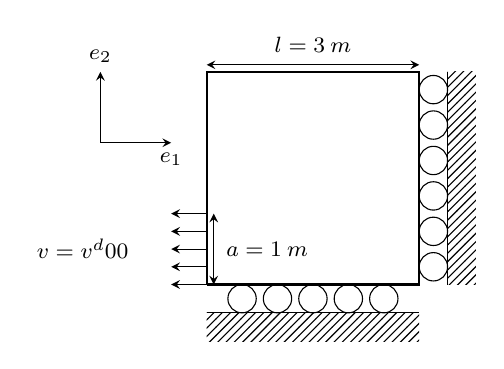
\begin{tikzpicture}[scale=0.9]
  \draw[thick] (0,0) --(3,0)--(3,3)--(0,3)--(0,0);
  \foreach \x in {0.5,1.,...,2.5} 
  \draw(\x,-0.2)circle(0.2);
  \foreach \x in {0.25,0.75,...,2.75} 
  \draw(3.2,\x)circle(0.2);
  \draw(0,-0.4)--(3.,-0.4);
  \draw(3.4,0)--(3.4,3);
  \fill [pattern=north east lines](0.0,-0.8)rectangle+(3,0.4);
  \fill [pattern=north east lines](3.4,0.)rectangle+(0.4,3);
  \draw[>=stealth,<->](0,3.1)--node[above=1pt]{\footnotesize $l=3 \: m$}(3,3.1);
  \draw[>=stealth,<->](0.1,0)--node[right=1pt]{\footnotesize $a=1 \: m$}(0.1,1);
  \foreach \x in {0.,0.25,...,1} 
  \draw[>=stealth,<-] (-0.5,\x)--(0.,\x);
  \node(a)at(-1.75,0.5){\footnotesize $\vect{v}=\matrice{v^d\\0 \\0}$}; 
  \draw[>=stealth,->](-1.5,2)--(-0.5,2)node(a)[anchor=north]{\footnotesize $\vect{e}_1$};
  \draw[>=stealth,->](-1.5,2)--(-1.5,3)node(a)[anchor=south]{\footnotesize $\vect{e}_2$};
\end{tikzpicture}


%%% Local Variables:
%%% mode: latex
%%% TeX-master: "../../aRenaud"
%%% End:

    \end{center}

    \onslide<2>
    \vspace{0.cm}
    \begin{center}
      % \movie[width=1.\linewidth,showcontrols,loop]{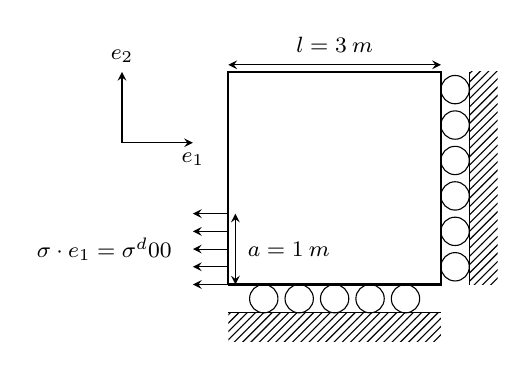
\begin{tikzpicture}[scale=0.9]
  \draw[thick] (0,0) --(3,0)--(3,3)--(0,3)--(0,0);
  \foreach \x in {0.5,1.,...,2.5} 
  \draw(\x,-0.2)circle(0.2);
  \foreach \x in {0.25,0.75,...,2.75} 
  \draw(3.2,\x)circle(0.2);
  \draw(0,-0.4)--(3.,-0.4);
  \draw(3.4,0)--(3.4,3);
  \fill [pattern=north east lines](0.0,-0.8)rectangle+(3,0.4);
  \fill [pattern=north east lines](3.4,0.)rectangle+(0.4,3);
  \draw[>=stealth,<->](0,3.1)--node[above=1pt]{\footnotesize $l=3 \: m$}(3,3.1);
  \draw[>=stealth,<->](0.1,0)--node[right=1pt]{\footnotesize $a=1 \: m$}(0.1,1);
  \foreach \x in {0.,0.25,...,1} 
  \draw[>=stealth,<-] (-0.5,\x)--(0.,\x);
  \node(a)at(-1.75,0.5){\footnotesize $\tens{\sigma}\cdot\vect{e}_1=\matrice{\sigma^d\\0 \\0}$}; 
  \draw[>=stealth,->](-1.5,2)--(-0.5,2)node(a)[anchor=north]{\footnotesize $\vect{e}_1$};
  \draw[>=stealth,->](-1.5,2)--(-1.5,3)node(a)[anchor=south]{\footnotesize $\vect{e}_2$};
\end{tikzpicture}


%%% Local Variables:
%%% mode: latex
%%% TeX-master: "../../mainManuscript"
%%% End:
}{section4/animation/hyperelasticity_velo/video.mp4}
      \movie[height = 0.7\paperheight,width=\linewidth, showcontrols,loop,poster,autostart]{%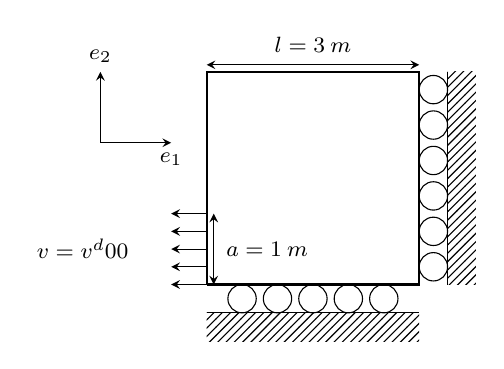
\begin{tikzpicture}[scale=0.9]
  \draw[thick] (0,0) --(3,0)--(3,3)--(0,3)--(0,0);
  \foreach \x in {0.5,1.,...,2.5} 
  \draw(\x,-0.2)circle(0.2);
  \foreach \x in {0.25,0.75,...,2.75} 
  \draw(3.2,\x)circle(0.2);
  \draw(0,-0.4)--(3.,-0.4);
  \draw(3.4,0)--(3.4,3);
  \fill [pattern=north east lines](0.0,-0.8)rectangle+(3,0.4);
  \fill [pattern=north east lines](3.4,0.)rectangle+(0.4,3);
  \draw[>=stealth,<->](0,3.1)--node[above=1pt]{\footnotesize $l=3 \: m$}(3,3.1);
  \draw[>=stealth,<->](0.1,0)--node[right=1pt]{\footnotesize $a=1 \: m$}(0.1,1);
  \foreach \x in {0.,0.25,...,1} 
  \draw[>=stealth,<-] (-0.5,\x)--(0.,\x);
  \node(a)at(-1.75,0.5){\footnotesize $\vect{v}=\matrice{v^d\\0 \\0}$}; 
  \draw[>=stealth,->](-1.5,2)--(-0.5,2)node(a)[anchor=north]{\footnotesize $\vect{e}_1$};
  \draw[>=stealth,->](-1.5,2)--(-1.5,3)node(a)[anchor=south]{\footnotesize $\vect{e}_2$};
\end{tikzpicture}


%%% Local Variables:
%%% mode: latex
%%% TeX-master: "../../aRenaud"
%%% End:

      }{section4/animation/hyperelasticity_velo/video.mp4}
    \end{center}
  \end{overprint}
\end{frame}


%%% Local Variables:
%%% mode: latex
%%% TeX-master: "../aRenaud"
%%% End:




%%% Local Variables:
%%% mode: latex
%%% TeX-master: "../aRenaud"
%%% End:




\part{Two-dimensional elastoplastic hyperbolic problems}\label{part:part2}
\section{Plastic waves}


\subsection{Historical review}
%% Problèmes traités -- approche expérimentale pour la confirmation
%% Type de solutions
%% Simple waves even for linear hardening in contrast to one-dimensional problems

\begin{frame}{Thin-walled tube problem}%{Historical review}
  \begin{columns}
    \begin{column}{0.4\textwidth}
      \begin{block}{\footnotesize Semi-infinite medium}
        % \centering
        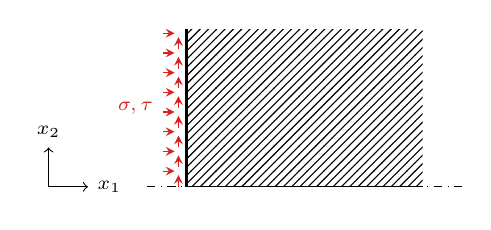
\begin{tikzpicture}
          \begin{scope}[shift={(-1.75,0)}]
            \draw[->] (0,0) -- (0.5,0) node[right] {\scriptsize $x_1$};
            \draw[->] (0,0) -- (0,0.5) node[above] {\scriptsize $x_2$};
          \end{scope}
          \draw (0,0) -- (3,.0);
          \draw[very thick] (0,0) -- (0,2.);
          \fill [pattern=north east lines] (0,0) rectangle (3.,2.);
          \draw[dash dot] (-0.5,0) -- (3.5,0);% node[right] {\footnotesize $x_1$};
          % \draw[->,dash dot] (0,0) -- (0,2.5) node[above] {\footnotesize $x_2$};
          \foreach \y in {0,0.25,...,1.75}
          \draw[Red,->,>=stealth] (-0.1,\y) -- (-0.1,\y+0.15);
          \foreach \y in {0,0.25,...,1.75}
          \draw[Red,->,>=stealth] (-0.30,\y+0.20) -- (-0.15,\y+0.20);
          \node[Red,left] at (-0.3,1.) {\scriptsize $\sigma,\tau$};
        \end{tikzpicture}  
      \end{block}
    \end{column}
    \begin{column}{0.52\textwidth}
      \begin{footnotesize}
        \begin{block}{\footnotesize Elastic-\alert{plastic} solution \cite{CRISTESCU19591605,Rakhmatulin}}
          \begin{columns}
            \begin{column}{0.25\textwidth}
              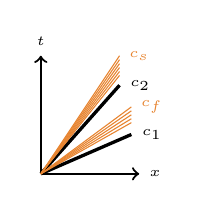
\begin{tikzpicture}[scale=0.5]
                \draw[thick,->] (-0.,0) -- (2.5,0) node[right] {\tiny $x$};
                \draw[thick,->] (-0.,-0.) -- (0,3) node[above] {\tiny $t$};
                \draw[very thick] (0,0) -- (2.3,1.) node[right] {\tiny $c_1$};
                % \draw[very thick] (0,0) -- (-2.3,1.) node[left] {\tiny $-c_1$};
                \draw[very thick] (0,0) -- (2.,2.25) node[right] {\tiny $c_2$};
                % \draw[very thick] (0,0) -- (-2.,2.25) node[left] {\tiny $-c_2$};
                \foreach \x in {1.3,1.4,1.5,1.6,1.7}
                {\draw[Orange] (0,0)-- (2.3,\x);
                  % \draw[Orange] (0,0)-- (-2.3,\x);
                }
                \node[Orange,right] at (2.3,1.7) {\tiny $c_f$};
                % \node[Orange,left] at (-2.3,1.7) {\tiny $-c_f$};
                \foreach \x in {2.5,2.6,2.7,2.8,2.9,3.}
                {\draw[Orange] (0,0)-- (2,\x);
                  % \draw[Orange] (0,0)-- (-2,\x);
                }
                \node[Orange,right] at (2,3) {\tiny $c_s$};
                % \node[Orange,left] at (-2,3) {\tiny $-c_s$};
              \end{tikzpicture}
            \end{column}
            \begin{column}{0.7\textwidth}
              \begin{itemize}
              \item[] fast and slow simple waves: $c_f,c_s$
              \item[] combined-stress waves
              \end{itemize}
            \end{column}
          \end{columns}
        \end{block}
      \end{footnotesize}
    \end{column}
  \end{columns}
  % Governing equations based on elastic-plastic softenesses
  \footnoteCite{CRISTESCU19591605,Rakhmatulin}
\end{frame}


\begin{frame}{Thin-walled tube problem: characteristic analysis \cite{Clifton}}
  %% Détailler travaux de clifton, comment il en arrive à des trajets élémentaires
  %% Problème de Picard
  \begin{footnotesize}
    \begin{columns}
      \begin{column}{0.6\textwidth}
        \begin{itemize}
          % \item ODEs governing the evolution of stress and velocity through both simple waves
        \item[] ODEs through simple waves: $d\tau=\psi(\tens{\sigma})d\sigma \rightarrow$ loading paths 
          \begin{itemize}
          \item \footnotesize characteristic structure not known a priori%integration: loading paths
          \item \footnotesize mathematical study $\rightarrow$ solution of Picard's problem
            % \centering
            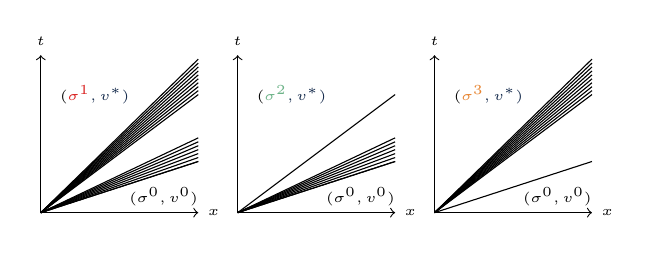
\begin{tikzpicture}
              \draw[->] (0,0) -- (2,0) node[right] {\tiny $x$};
              \draw[->] (0,0) -- (0,2) node[above] {\tiny $t$};
              \node[right] at (1,0.2) {\tiny $(\tens{\sigma}^0,\vect{v}^0)$};
              \draw (0,0) -- (2,0.65);
              \foreach \y in {0.65,0.7,...,1.}
              \draw (0,0) -- (2,\y);
              \foreach \y in {1.5,1.55,...,2.}
              \draw (0,0) -- (2,\y);
              \node[left] at (1.25,1.5) {\tiny $(\color{Red}\tens{\sigma}^1\color{CNBlue},\vect{v}^*)$};
              \begin{scope}[shift={(2.5,0)}]
                \draw[->] (0,0) -- (2,0) node[right] {\tiny $x$};
                \draw[->] (0,0) -- (0,2) node[above] {\tiny $t$};
                \node[right] at (1,0.2) {\tiny $(\tens{\sigma}^0,\vect{v}^0)$};
                \draw (0,0) -- (2,0.65);
                \foreach \y in {0.65,0.7,...,1.}
                \draw (0,0) -- (2,\y);
                % \foreach \y in {1.5,1.55,...,2.}
                % \draw (0,0) -- (2,\y);
                \draw (0,0) -- (2,1.5);
                \node[left] at (1.25,1.5) {\tiny $(\color{Green}\tens{\sigma}^2\color{CNBlue},\vect{v}^*)$};
              \end{scope}
              \begin{scope}[shift={(5,0)}]
                \draw[->] (0,0) -- (2,0) node[right] {\tiny $x$};
                \draw[->] (0,0) -- (0,2) node[above] {\tiny $t$};
                \node[right] at (1,0.2) {\tiny $(\tens{\sigma}^0,\vect{v}^0)$};
                \draw (0,0) -- (2,0.65);
                \foreach \y in {1.5,1.55,...,2.}
                \draw (0,0) -- (2,\y);
                \node[left] at (1.25,1.5) {\tiny $(\color{Orange}\tens{\sigma}^3\color{CNBlue},\vect{v}^*)$};
              \end{scope}
            \end{tikzpicture}
          \item \footnotesize iterative Riemann solver \cite{Lin_et_Ballman}
          \end{itemize}
        \end{itemize}
      \end{column}
      \begin{column}{0.43\textwidth}
        \begin{overprint}
          \onslide<1>
          \vskip 5pt
          \centering
          \begin{tikzpicture}[scale=0.7]
  \begin{axis}[ymajorgrids=true,xmajorgrids=true,ylabel=$\tau \: (Pa)$,xlabel=$\sigma \: (Pa)$,xmin=-0.1e8,xmax=2.e8,ymin=0.,ymax=7.5e7]
    %%
    \addplot[very thick] table [x=sigma_11,y=sigma_12] {section5/pgfFigures/pgf_thinWalledTubeSlowWave/TWslowStressPlane_Stress0.pgf};
    %%
    \addplot[very thick] table [x=sigma_11,y=sigma_12] {section5/pgfFigures/pgf_thinWalledTubeSlowWave/TWslowStressPlane_Stress1.pgf};
    %%
    \addplot[very thick] table [x=sigma_11,y=sigma_12] {section5/pgfFigures/pgf_thinWalledTubeSlowWave/TWslowStressPlane_Stress2.pgf};
    %%
    \addplot[very thick] table [x=sigma_11,y=sigma_12] {section5/pgfFigures/pgf_thinWalledTubeSlowWave/TWslowStressPlane_Stress3.pgf};
    %%
    \addplot[very thick] table [x=sigma_11,y=sigma_12] {section5/pgfFigures/pgf_thinWalledTubeSlowWave/TWslowStressPlane_Stress4.pgf};
    %%
    \addplot[very thick] table [x=sigma_11,y=sigma_12] {section5/pgfFigures/pgf_thinWalledTubeSlowWave/TWslowStressPlane_Stress5.pgf};
    %%
    \addplot[very thick] table [x=sigma_11,y=sigma_12] {section5/pgfFigures/pgf_thinWalledTubeSlowWave/TWslowStressPlane_Stress6.pgf};
    %% Yield surface
    \addplot[black,dashed] table  [x=sigma_11,y=sigma_12] {section5/pgfFigures/pgf_thinWalledTubeSlowWave/TWslow_yield0.pgf};

    %\addplot[very thick,Orange,restrict y to domain=4.e7:6.75e7] table [x=sigma_11,y=sigma_12]{section5/pgfFigures/pgf_thinWalledTubeSlowWave/TWslowStressPlane_Stress1.pgf};


  \end{axis}
\end{tikzpicture}

%%% Local Variables:
%%% mode: latex
%%% TeX-master: "../../presentation"
%%% End:
          \onslide<2>
          \vskip 5pt
          \centering
          \begin{tikzpicture}[scale=0.7]
  \begin{axis}[ymajorgrids=true,xmajorgrids=true,ylabel=$\tau \: (Pa)$,xlabel=$\sigma \: (Pa)$,xmin=-0.1e8,xmax=1.5e8,ymin=0.,ymax=7.5e7, legend pos=north east]
    %% Yield surface
    \addplot[black,densely dotted] table  [x=sigma_11,y=sigma_12] {section5/pgfFigures/pgf_thinWalledTubeSlowWave/TWslow_yield0.pgf};
    \addlegendentry{yield surface}
    %%
    \addplot[black,loosely dashed,thick] table  [x=sigma_11,y=sigma_12] {section5/pgfFigures/pgf_thinWalledTubeSlowWave/TWslow_yield0.pgf};
    \addlegendentry{fast wave}
    %% 
    \addplot[very thick] table [x=sigma_11,y=sigma_12] {section5/pgfFigures/pgf_thinWalledTubeSlowWave/TWslowStressPlane_Stress0.pgf};
    \addlegendentry{slow wave}
    %%
    \addplot[very thick] table [x=sigma_11,y=sigma_12] {section5/pgfFigures/pgf_thinWalledTubeSlowWave/TWslowStressPlane_Stress1.pgf};
    %%
    \addplot[very thick] table [x=sigma_11,y=sigma_12] {section5/pgfFigures/pgf_thinWalledTubeSlowWave/TWslowStressPlane_Stress2.pgf};
    %%
    \addplot[very thick] table [x=sigma_11,y=sigma_12] {section5/pgfFigures/pgf_thinWalledTubeSlowWave/TWslowStressPlane_Stress3.pgf};
    %%
    \addplot[very thick] table [x=sigma_11,y=sigma_12] {section5/pgfFigures/pgf_thinWalledTubeSlowWave/TWslowStressPlane_Stress4.pgf};
    %%
    \addplot[very thick] table [x=sigma_11,y=sigma_12] {section5/pgfFigures/pgf_thinWalledTubeSlowWave/TWslowStressPlane_Stress5.pgf};
    %%
    \addplot[very thick] table [x=sigma_11,y=sigma_12] {section5/pgfFigures/pgf_thinWalledTubeSlowWave/TWslowStressPlane_Stress6.pgf};
    %% Yield surface
    \addplot[black,dashed] table  [x=sigma_11,y=sigma_12] {section5/pgfFigures/pgf_thinWalledTubeSlowWave/TWslow_yield0.pgf};

    \addplot[very thick,Red,restrict x to domain=0.2e8:0.5e8] table [x=sigma_11,y=sigma_12]{section5/pgfFigures/pgf_thinWalledTubeSlowWave/TWslow_yield0.pgf};
    \addplot[very thick,Red,restrict y to domain=4.e7:6.5e7] table [x=sigma_11,y=sigma_12] {section5/pgfFigures/pgf_thinWalledTubeSlowWave/TWslowStressPlane_Stress2.pgf};

    \node[right] at (axis cs:0.55e8,6.5e7) {$\color{Red}\tens{\sigma}^1$};
  \end{axis}
\end{tikzpicture}

%%% Local Variables:
%%% mode: latex
%%% TeX-master: "../../presentation"
%%% End:
          \onslide<3>
          \vskip 5pt
          \centering
          \begin{tikzpicture}[scale=0.7]
  \begin{axis}[ymajorgrids=true,xmajorgrids=true,ylabel=$\tau \: (Pa)$,xlabel=$\sigma \: (Pa)$,xmin=-0.1e8,xmax=1.5e8,ymin=0.,ymax=7.5e7, legend pos=north east]
    %% Yield surface
    \addplot[black,densely dotted] table  [x=sigma_11,y=sigma_12] {section5/pgfFigures/pgf_thinWalledTubeSlowWave/TWslow_yield0.pgf};
    \addlegendentry{yield surface}
    %%
    \addplot[black,loosely dashed,thick] table  [x=sigma_11,y=sigma_12] {section5/pgfFigures/pgf_thinWalledTubeSlowWave/TWslow_yield0.pgf};
    \addlegendentry{fast wave}
    %%
    \addplot[very thick] table [x=sigma_11,y=sigma_12] {section5/pgfFigures/pgf_thinWalledTubeSlowWave/TWslowStressPlane_Stress0.pgf};
    \addlegendentry{slow wave}
    %%
    \addplot[very thick] table [x=sigma_11,y=sigma_12] {section5/pgfFigures/pgf_thinWalledTubeSlowWave/TWslowStressPlane_Stress1.pgf};
    %%
    \addplot[very thick] table [x=sigma_11,y=sigma_12] {section5/pgfFigures/pgf_thinWalledTubeSlowWave/TWslowStressPlane_Stress2.pgf};
    %%
    \addplot[very thick] table [x=sigma_11,y=sigma_12] {section5/pgfFigures/pgf_thinWalledTubeSlowWave/TWslowStressPlane_Stress3.pgf};
    %%
    \addplot[very thick] table [x=sigma_11,y=sigma_12] {section5/pgfFigures/pgf_thinWalledTubeSlowWave/TWslowStressPlane_Stress4.pgf};
    %%
    \addplot[very thick] table [x=sigma_11,y=sigma_12] {section5/pgfFigures/pgf_thinWalledTubeSlowWave/TWslowStressPlane_Stress5.pgf};
    %%
    \addplot[very thick] table [x=sigma_11,y=sigma_12] {section5/pgfFigures/pgf_thinWalledTubeSlowWave/TWslowStressPlane_Stress6.pgf};
    %% Yield surface
    \addplot[black,dashed] table  [x=sigma_11,y=sigma_12] {section5/pgfFigures/pgf_thinWalledTubeSlowWave/TWslow_yield0.pgf};

    \addplot[very thick,Green,restrict x to domain=0.4e8:0.95e8,arrows along my path] table [x=sigma_11,y=sigma_12]{section5/pgfFigures/pgf_thinWalledTubeSlowWave/TWslow_yield0.pgf};

    \addplot[very thick,Green,arrows along my path] coordinates{(0.42e8,5.25e7) (0.42e8,0.) (0,0)  };
    
    \node[right] at (axis cs:0.95e8,1.8e7) {$\color{Green}\tens{\sigma}^2$};
  \end{axis}
\end{tikzpicture}

%%% Local Variables:
%%% mode: latex
%%% TeX-master: "../../presentation"
%%% End:
          \onslide<4>
          \vskip 5pt
          \centering
          \begin{tikzpicture}[scale=0.7]
  \begin{axis}[ymajorgrids=true,xmajorgrids=true,ylabel=$\tau \: (Pa)$,xlabel=$\sigma \: (Pa)$,xmin=-0.1e8,xmax=1.5e8,ymin=0.,ymax=7.5e7, legend pos=north east]
    %% Yield surface
    \addplot[black,densely dotted] table  [x=sigma_11,y=sigma_12] {section5/pgfFigures/pgf_thinWalledTubeSlowWave/TWslow_yield0.pgf};
    \addlegendentry{yield surface}
    %%
    \addplot[black,loosely dashed,thick] table  [x=sigma_11,y=sigma_12] {section5/pgfFigures/pgf_thinWalledTubeSlowWave/TWslow_yield0.pgf};
    \addlegendentry{fast wave}
    %% 
    \addplot[very thick] table [x=sigma_11,y=sigma_12] {section5/pgfFigures/pgf_thinWalledTubeSlowWave/TWslowStressPlane_Stress0.pgf};
    \addlegendentry{slow wave}
    %%
    \addplot[very thick] table [x=sigma_11,y=sigma_12] {section5/pgfFigures/pgf_thinWalledTubeSlowWave/TWslowStressPlane_Stress1.pgf};
    %%
    \addplot[very thick] table [x=sigma_11,y=sigma_12] {section5/pgfFigures/pgf_thinWalledTubeSlowWave/TWslowStressPlane_Stress2.pgf};
    %%
    \addplot[very thick] table [x=sigma_11,y=sigma_12] {section5/pgfFigures/pgf_thinWalledTubeSlowWave/TWslowStressPlane_Stress3.pgf};
    %%
    \addplot[very thick] table [x=sigma_11,y=sigma_12] {section5/pgfFigures/pgf_thinWalledTubeSlowWave/TWslowStressPlane_Stress4.pgf};
    %%
    \addplot[very thick] table [x=sigma_11,y=sigma_12] {section5/pgfFigures/pgf_thinWalledTubeSlowWave/TWslowStressPlane_Stress5.pgf};
    %%
    \addplot[very thick] table [x=sigma_11,y=sigma_12] {section5/pgfFigures/pgf_thinWalledTubeSlowWave/TWslowStressPlane_Stress6.pgf};
    %% Yield surface
    \addplot[black,dashed] table  [x=sigma_11,y=sigma_12] {section5/pgfFigures/pgf_thinWalledTubeSlowWave/TWslow_yield0.pgf};

    
    \addplot[very thick,Orange,restrict y to domain=4.e7:6.75e7] table [x=sigma_11,y=sigma_12]{section5/pgfFigures/pgf_thinWalledTubeSlowWave/TWslowStressPlane_Stress1.pgf};
    \addplot[very thick,Orange,arrows along my path] coordinates{(0.25e8,5.6e7) (0.25e8,0.) (0,0)};
    
    \node[right] at (axis cs:0.25e8,6.75e7) {$\color{Orange}\tens{\sigma}^3$};
  \end{axis}
\end{tikzpicture}

%%% Local Variables:
%%% mode: latex
%%% TeX-master: "../../presentation"
%%% End:
        \end{overprint}
        
      \end{column}
    \end{columns}
  \end{footnotesize}
  % \cite{Clifton,Clifton_exp}
  \footnoteCite{Clifton,Lin_et_Ballman}
\end{frame}

\subsection{General formulation}
\begin{frame}
  \begin{block}{Problems tackled overall}
    \begin{itemize}
    \item Particular plane strain and plane stress cases \cite{Bleich,Ting69,Ting73,Li_planeStress_EP}
    \item Equations based on elastic-plastic compliances
    
    \end{itemize}
  \end{block}
  \begin{block}{The proposed approach}
    Hyperbolic system in the arbitrary direction $\vect{n}$: $\drond{\Qcb}{t} + \Jbsf \drond{\Qcb}{x_n} =\vect{0}$ \\
    $\Jbsf=-\matrice{\tens{0}^2 & \frac{1}{\rho}\tens{I}\otimes\vect{n} \\ \alert{\Cbb^{ep}\cdot \vect{n}} & \tens{0}^4}$
    \begin{itemize}
    \item General plane strain and plane stress problems \textbf{under small strains}
    \item Unified framework
    % \item generalizes to plane strain and plane stress problems
    \end{itemize}
  \end{block}
  \footnoteCite{Bleich,Ting69,Ting73,Li_planeStress_EP}
\end{frame}

% \begin{frame}
  % \begin{block}{Governing equations}
  %   \begin{footnotesize}
  %     \begin{columns}
  %       \begin{column}{0.4\textwidth}
  %         \begin{flalign*}
  %           & \text{plastic flow: } \dot{\tens{\eps}}^p = \dot{p}\drond{f}{\tens{\sigma}} \\
  %           & \text{constitutive equations: } \dot{\tens{\sigma}}=\Cbb^{ep}:\dot{\tens{\eps}} \\
  %           & \text{linear momentum: } \drond{\rho \vect{v}}{t} - \nabla_v \cdot\tens{\sigma} = \vect{0}\\
  %           & \text{kinematic laws: } \dot{\tens{\eps}} = \nablat^s \vect{v}
  %         \end{flalign*}
  %       \end{column}
  %       \begin{column}{0.55\textwidth}
  %         \begin{flalign*}
  %           \Rightarrow \: &\text{quasi-linear form: } \drond{\Ucb}{\Qcb}\drond{\Qcb}{t} + \drond{\Fcb\cdot\vect{e}_i}{\Qcb}\drond{\Qcb}{x_i}=\vect{0} \\
  %           & \Ucb = \matrice{\rho \vect{v} \\ \tens{\eps}} \: ; \: \Qcb = \matrice{\vect{v} \\ \tens{\sigma}} \: ;\: \Fcb \cdot \vect{e}_i = -\matrice{\sigma_{ji}  \\ \frac{v_j \delta_{ik} + v_i \delta_{jk}}{2}}, (i,j,k) = \{1,2,3\}
  %         \end{flalign*}
  %       \end{column}
  %     \end{columns}
  %     %Difference with previous formulations ? Inverse $\drond{\Ucb}{\Qcb}$ rather than its matrix representation $\rightarrow$ stiffnesses instead of softenesses
  %     %% system kept generical so far
  %   \end{footnotesize}
  %   \begin{block}{Hyperbolic system in the arbitrary direction $\vect{n}$}
  %     \begin{flalign*}
  %       \drond{\Qcb}{t} + \Jbsf \drond{\Qcb}{x_n} =\vect{0}
  %     \end{flalign*}
  %     with the Jacobian matrix $\Jbsf=-\matrice{\tens{0}^2 & \frac{1}{\rho}\tens{I}\otimes\vect{n} \\ \alert{\Cbb^{ep}\cdot \vect{n}} & \tens{0}^4}$
  %   \end{block}
  % \end{block}
% \end{frame}



%%% Local Variables:
%%% mode: latex
%%% TeX-master: "../presentation"
%%% End:


\section{Loading paths through plastic waves}

\section{Numerical results}



\end{document}

%%% Local Variables:
%%% mode: latex
%%% TeX-master: t
%%% End:
